\documentclass[aspectratio=169]{beamer}

\usepackage{xcolor}
\usepackage{tikz}
\usetikzlibrary{shapes.arrows}
\usepackage{stackrel}
\usepackage{bm,bbm}% bold math
\usepackage[version=3]{mhchem}
\usepackage{lmodern}

\usepackage{multirow}
\usepackage{setspace}
\usepackage{yfonts}
\usepackage{mathrsfs}
\usepackage[most]{tcolorbox}
\usepackage{colortbl}
\usepackage{commath}
\usepackage{empheq}
\usepackage{multicol}
\usepackage{mhchem}
\usepackage[normalem]{ulem}
\usepackage{pifont}
\usepackage{fontawesome}
\usepackage{listings}

% Support for Pandoc-beamer
\usepackage[T1]{fontenc}
\usepackage{booktabs}
\usepackage{longtable}
\usepackage{fancyvrb}
\providecommand{\tightlist}{%
  \setlength{\itemsep}{0pt}\setlength{\parskip}{0pt}}

\usepackage[retainorgcmds]{IEEEtrantools}
\usepackage{siunitx}
\sisetup{detect-display-math=true,detect-weight=true,detect-family=true}

\usepackage{tcolorbox,xcolor,framed}
\DefineVerbatimEnvironment{Highlighting}{Verbatim}{fontsize=\footnotesize,commandchars=\\\{\}}
\definecolor{shadecolor}{rgb}{0.9,0.9,0.9}
\newenvironment{Shaded}{\snugshade}{\endsnugshade}
\newcommand{\KeywordTok}[1]{\textcolor[rgb]{0.13,0.29,0.53}{\textbf{#1}}}
\newcommand{\DataTypeTok}[1]{\textcolor[rgb]{0.13,0.29,0.53}{#1}}
\newcommand{\NormalTok}[1]{#1}
\newcommand{\DecValTok}[1]{\textcolor[rgb]{0.00,0.00,0.81}{#1}}
\newcommand{\CommentTok}[1]{\textcolor[rgb]{0.56,0.35,0.01}{\textit{{#1}}}}
\newcommand{\PreprocessorTok}[1]{\textcolor[rgb]{0.56,0.35,0.01}{\textit{{#1}}}}
\newcommand{\ControlFlowTok}[1]{\textcolor[rgb]{0.13,0.29,0.53}{\textbf{{#1}}}}


\usepackage[colorinlistoftodos, color=blue!20!white, bordercolor=gray,
textsize=tiny]{todonotes}

\setbeamercolor{structure}{fg=myOrange}
\setbeamercolor{normal text}{fg=myBlue}

\makeatletter
\newcommand*{\overlaynumber}{\number\beamer@slideinframe}
\makeatother

\usepackage{pgf}
\usetikzlibrary{arrows,shapes,shapes.arrows,positioning,calc,decorations.text}

\usepackage{standalone}

\usetheme{default}

\usepackage{multimedia}
\usepackage{graphicx}
\usepackage{animate}
% \usepackage{minted}
\usepackage{animate}


\definecolor{RED}{RGB}{255,0,0}  %%%
\definecolor{myBlue}{RGB}{19,41,75}  %%% BLUE
\definecolor{myBlueLink}{RGB}{70,70,200}  %%% LINK BLUE
\definecolor{myOrange}{RGB}{232,74,39}   %%% ILLINOIS ORANGE
\definecolor{IllinoisOrange}{RGB}{232,74,39}  %%% ILLINOIS ORANGE
\definecolor{IllinoisBlue}{RGB}{19,41,75}   %%% ILLINOIS BLUE
\definecolor{mainTextColor}{RGB}{19,41,75}  %%% ILLINOIS BLUE
\definecolor{myLightGray}{rgb}{0.95,0.95,0.95}
\definecolor{myGold}{rgb}{1.0,.75,0.0}


%%% Modify the footline to only have the page numbering in the center, nothing else
\makeatletter
\setbeamertemplate{footline}
{
 \leavevmode%
 \hbox{\begin{beamercolorbox}[wd=\paperwidth,ht=2.25ex,dp=1ex]{}%
     \usebeamerfont{author in head/foot}%
     \hspace*{0.02in}
     \raisebox{-0.0in}{
\includegraphics[height=0.21in]{../UILogoBlockI.pdf}}%
     \hfill\hspace*{0.8in}\insertframenumber{}
     \hfill\raisebox{-0.07in}{
\includegraphics[height=0.3in]{../ceesd-logo-2.pdf}}%
 \end{beamercolorbox}}
 \vskip0pt%
}

%%% Modify the headline to be null
\setbeamertemplate{headline}{}

%%% Set frame title to be transparent with black text
\setbeamercolor{frametitle}{bg=}
\setbeamercolor{frametitle}{fg=myOrange}


%%% Set frame title to properly center the text
\setbeamertemplate{frametitle}
{
  \leavevmode%
  \hbox{%
  \begin{beamercolorbox}[wd=\paperwidth,ht=2.5ex,dp=0ex]{frametitle}%
    \raggedright
    \bfseries
    \hspace*{0.3em}%
    \usebeamerfont{frametitle}\insertframetitle
  \end{beamercolorbox}}
  \vspace*{-2.75ex}
}


\makeatother

\setbeamersize{text margin left=0.15in,text margin right=0.15in}

%%% turn off navigation line (uncomment to reinstate)
\setbeamertemplate{navigation symbols}{}

%%% turn off the balls for enumerate
\setbeamertemplate{enumerate items}[default]
% \setbeamertemplate{itemize items}[default]

\setbeamertemplate{itemize subitem}{$\bullet$}
\setbeamertemplate{itemize subsubitem}{$*$}


%%% Set the background image
% \usebackgroundtemplate%
% {%
%     
\includegraphics[width=\paperwidth]{../ceesd-slide-background.pdf}%
% }



\def\Put(#1,#2)#3{\leavevmode\makebox(0,0){\put(#1,#2){#3}}}
\newcommand{\prj}[2]{{\color{gray} #1 [#2]}}
\newcommand{\noprj}[2]{}
\newcommand{\talkref}[2]{{\color{gray} #1 [#2]}}
\newcommand{\makered}[1]{{\color{red} #1}}
\newcommand{\makeblue}[1]{{\color{blue} #1}}
\newcommand{\makecyan}[1]{{\color{cyan} #1}}
\newcommand{\makegreen}[1]{{\color{green} #1}}
\newcommand{\maketeal}[1]{{\color{teal} #1}}
\newcommand{\makeorange}[1]{{\color{orange} #1}}
\newcommand{\makeRed}[1]{{\color{red} #1}}
\newcommand{\makeBlue}[1]{{\color{blue} #1}}
\newcommand{\makeOrange}[1]{{\color{orange} #1}}
\newcommand{\makeGreen}[1]{{\color{ForestGreen} #1}}
\newcommand{\makeCyan}[1]{{\color{cyan} #1}}
\newcommand{\makeGold}[1]{{\color{myGold} #1}}

\newcommand{\clink}{{\tiny({\color{blue} link})}}


\newcommand{\myoul}[1]{\color{myBlue}\underline{\smash{\color{myOrange} #1}}\color{myOrange}}
\newcommand{\ccdot}{\color{myBlue}$\circ$\color{myOrange}\;}
\newcommand{\cc}[1]{\color{myBlue}#1\color{myOrange}{}}

\newcommand{\HRule}[2]{{\color{myBlue}\rule{#1}{#2}}}
\newcommand{\dRightarrow}{{\color{myOrange}\Rightarrow}}
\newcommand{\dLeftarrow}{{\color{myBlue}\Leftarrow}}
\newcommand{\tb}[1]{{\color{blue}(#1)}}
\newcommand{\tr}[1]{{\color{blue}({\color{red}#1})}}
\newcommand{\tor}[1]{{\color{blue}({\color{blue}#1})}}
\newcommand{\lead}[1]{\textit{\color{myBlue}(#1)}}
\newcommand{\bmath}{\boldsymbol}
\newcommand{\eps}{\varepsilon}
\newcommand{\vp}{\vec{p}}
\newcommand{\rPI}[1]{{\color{myOrange}#1}}
\newcommand{\tPI}[1]{\texttt{\color{myOrange}#1}}
\newcommand{\ttPI}[1]{\texttt{\color{myOrange}#1}}
\newcommand{\cPI}[1]{\textbf{\color{myOrange}#1}}
\newcommand{\iPI}[1]{\textit{\color{myOrange}#1}}
\newcommand{\sPI}[1]{\textsc{\color{myOrange}#1}}
\newcommand{\scPI}[1]{\textsc{\color{myOrange}#1}}
\newcommand{\tabtit}[1]{\textsc{\color{myOrange}#1}}
\newcommand{\Dpartial}[2]{\frac{\partial #1}{\partial #2}}
\newcommand{\bx}{\mathbf{x}}
\newcommand{\bU}{\mathbf{U}}
\newcommand{\obsigma}{{\bar \sigma}}
\newcommand{\bomega}{\boldsymbol{\omega}}
\newcommand{\vsigma}{\vec{\sigma}}
\newcommand{\II}{{I\!I}}
\newcommand{\memph}[1]{{\color{red} #1}}
\newcommand{\eg}{\emph{e.g.}}
\newcommand{\mat}[1]{\ensuremath{\mathsf{#1}}}
\newcommand{\bvec}[1]{\ensuremath{\boldsymbol{#1}}}



\newcommand{\sectionWithFrame}[1]{%
  \section{#1}
  \begin{frame}
    \centerline{\LARGE \insertsection}
  \end{frame}}
\newcommand{\sectionAndsubWithFrame}[2]{%
  \section{#1}
  \begin{frame}
    \begin{center}\LARGE #1\end{center}
    \bigskip
    \centerline{\large #2}
  \end{frame}}

\newcommand{\cM}{\mathcal{M}}

\newcommand{\bn}{\mathbf{n}}

\newcommand{\bbC}{\mathbb{C}}
\newcommand{\vbbm}{{\vec{m}}}
\newcommand{\bbM}{\mathbb{M}}
\newcommand{\bbH}{\mathbb{H}}
\newcommand{\bbG}{\mathbb{G}}
\newcommand{\bbV}{\mathbb{V}}

\newcommand{\vD}{{\vec D}}
\newcommand{\vhD}{{\hat{D}}}
\newcommand{\vg}{{\vec g}}
\newcommand{\vphi}{{\vec\phi}}
\newcommand{\vOmega}{{\vec\Omega}}

\newcommand{\vF}{{\vec{F}}}
\newcommand{\vf}{{\vec{f}}}
\newcommand{\vb}{{\vec{b}}}
\newcommand{\vh}{{\vec{h}}}
\newcommand{\vq}{{\vec{q}}}
\newcommand{\vqs}{{\vec{q}^{\,\color{red}*}}}

\newcommand{\cJ}{\mathcal{J}}
\newcommand{\cK}{\mathcal{K}}
\newcommand{\cG}{\mathcal{G}}
\newcommand{\cI}{\mathcal{I}}
\newcommand{\cP}{\mathcal{P}}
\newcommand{\cN}{\mathcal{N}}
\newcommand{\cC}{\mathcal{C}}
\newcommand{\cO}{\mathcal{O}}
\newcommand{\cS}{\mathcal{S}}
\newcommand{\cQ}{\mathcal{Q}}
\newcommand{\cR}{\mathcal{R}}

\newcommand{\rstar}{{\color{red}*}}
\newcommand{\rchk}{{\color{red} \checkmark}}
\newcommand{\rex}{{\color{red} \ding{55}}}
\newcommand{\gchk}{{\color{green} \checkmark}}
\newcommand{\obul}{{\color{orange} $\bullet$}}
\newcommand{\rbul}{{\color{red} $\bullet$}}
\newcommand{\pbul}{{\color{myBlue} $\bullet$}}
\newcommand{\ro}{{\color{red} $\circ$}}
\newcommand{\bd}{{\color{blue} $\bullet$}}
\newcommand{\po}{{\color{myOrange} $\circ$}}

\newcommand{\rhoi}[1][i]{\rho_{#1}}
\newcommand{\dt}[1][t]{\partial_{#1}}
\newcommand{\dx}[1][{\textrm{\bf x}}]{\boldsymbol \partial_{#1}}
\newcommand{\Vi}[1][i]{\mathcal{V}_{#1}}
\newcommand{\Mi}[1][\textswab{i}]{\mathcal{M}_{#1}}
\newcommand{\omegai}[1][i]{\dot{\omega}_{#1}}
\newcommand{\grav}{{\bf g}}
\newcommand{\Etot}{\mathcal{E}}

\newcommand{\mBG}{m_{\text{\tiny BG}}}
\newcommand{\nBG}{n_{\text{\tiny BG}}}
\newcommand{\nIp}{n_{\text{\tiny $I^+$}}}
\newcommand{\nIm}{n_{\text{\tiny $I^-$}}}


\newcommand{\bI}{{\mathbf{I}}}
\newcommand{\bq}{{\mathbf{q}}}
\newcommand{\btau}{{\boldsymbol{\tau}}}

\newcommand{\bv}{{\bar{v}}}
\newcommand{\bepsilon}{{\bar{\epsilon}}}

\newcommand{\ST}{{S_{\text{\tiny T}}}}

\newcommand{\vu}{\vec{u}}
\newcommand{\vQ}{\vec{Q}}
\newcommand{\veta}{\vec{\eta}}


  \newcommand{\Grad}{\bnabla}
  \newcommand{\Div}{\bnabla\vdot}
  \newcommand{\Curl}{\bnabla\vprod}
  \newcommand{\hGrad}{\bnabla^{}_{\!\!\mathrm{h}}}
  \newcommand{\hDiv}{\bnabla^{}_{\!\!\mathrm{h}}\!\vdot}
  \newcommand{\pGrad}{\bnabla^{}_{\!\!\!\perp}}
  \newcommand{\pDiv}{\bnabla^{}_{\!\!\!\perp}\!\vdot}
\newcommand{\pop}[2]{\frac{\partial #1}{\partial #2}}
\newcommand{\pp}[1]{\ensuremath{\left[ #1 \right]}}
\newcommand{\psq}[1]{\ensuremath{{\left[ #1 \right]}}}

% Grad, div, curl, etc.
\newcommand{\vdot}{\mathop{\mbox{\boldmath{$\cdot$}}}}
\newcommand{\vddot}{\mathop{\mbox{\textbf{:}}}}
\newcommand{\bnabla}{\mbox{\boldmath{$\nabla$}}}
\newcommand{\Lapl}{\nabla^2}
\newcommand{\hLapl}{\nabla^2_{\!\mathrm{h}}}
\newcommand{\pLapl}{\nabla^2_{\!\!\!\perp}}

\newcommand{\kION}{k_{\text{\tiny ION}}}
\newcommand{\kDET}{k_{\text{\tiny DET}}}
\newcommand{\kDR}{k_{\text{\tiny DR}}}
\newcommand{\kDA}{k_{\text{\tiny DA}}}
\newcommand{\kII}{k_{\text{\tiny $II$}}}


\def\colorize<#1>{%
\temporal<#1>{}{\color{red}}{}
}

\newcommand{\paper}[1]{ {\tiny #1\par} }
\newcommand{\TODO}[1]{{\color{red} \tiny TODO: #1}}
\newcommand{\CHK}{{\color{red} ???}}
\newcommand{\CHKWDG}{{\color{red} ???WDG???}}
\newcommand{\progname}[1]{\textit{#1}}
\newcommand{\PlasComCM}{\progname{PlasComCM}}
\newcommand{\PlasComCMtwo}{\progname{PlasCom2}}
\newcommand{\plascomtwo}{\progname{PlasCom2}}
\newcommand{\dancode}{\PlasComCM}
\newcommand{\dancodetwo}{\progname{PlasCom2}}
\newcommand{\codelet}[1]{\progname{Codelet-#1}}
\newcommand{\goldenCopy}{\rPI{golden copy}}
\newcommand{\GoldenCopy}{\rPI{Golden copy}}
\newcommand{\code}[1]{\texttt{#1}}
\newcommand{\PCtwo}{\progname{PlasCom2}}
\newcommand{\CSTUF}{\progname{CSTUF}}
\newcommand{\mirgecom}{\progname{MIRGE-Com}}
\newcommand{\pyrometheus}{\progname{Pyrometheus}}
\newcommand{\mirgeheat}{\progname{MIRGE-Heat}}
\newcommand{\plusplus}[1]{#1{}\texttt{++}}
\newcommand{\ceesdcode}{\textit{MIRGE-Com}}
\newcommand{\ceesdMIRGE}{\textit{MIRGE}}

\newcommand{\xnew}{$^{\text{\tiny \makered{new}}}$}
\newcommand{\xremind}{$^{\text{\tiny \makeblue{reminder}}}$}
\newcommand{\Q}[1]{{\medskip\small\noindent\color{blue!60!white}#1\par}}

\newcommand{\insertmovie}[3]{\ifmovies{
\movie[autostart,loop]
{\includegraphics[width=#1\textwidth]{Movies/#2}}
{Movies/#3}
}
\else{
\includegraphics[width=#1\textwidth]{Movies/#2}
}
\fi
}

\usefonttheme[onlymath]{serif}

\definecolor{ForestGreen}{rgb}{0.0, 0.2, 0.13}
\definecolor{darkpastelgreen}{rgb}{0.01, 0.75, 0.24}
\definecolor{antiquewhite}{rgb}{0.98, 0.92, 0.84}

\newcommand{\planA}{$\mathbb{A}$}
\newcommand{\planAA}{$\mathcal{A}'$}
\newcommand{\planB}{B}

\newcommand{\MUST}{{\footnotesize\color{red} \textbf{MUST}}}
\newcommand{\WISH}{{\footnotesize\color{orange} \textbf{WISH}}}
\newcommand{\DEFER}{{\footnotesize\color{yellow} \textbf{DEFER}}}
\newcommand{\MAYBE}{{\footnotesize\color{lightgray} \textbf{MAYBE}}}
\newcommand{\RETURN}{{\footnotesize\color{blue} \textbf{RETURN}}}
\newcommand{\DONE}{{\footnotesize\color{ForestGreen} \textbf{DONE}}}
\newcommand{\PLAN}{{\footnotesize\color{green} \textbf{PLANNED}}}
\newcommand{\CURRENT}{{\footnotesize\color{cyan} \textbf{NOW}}}

\newcommand{\SNL}{{\footnotesize $\;\rightarrow$ SNL}}
\newcommand{\LLNL}{{\footnotesize $\;\rightarrow$ LLNL}}
\newcommand{\LANL}{{\footnotesize $\;\rightarrow$ LANL}}


\newcommand{\aMUST}{\tiny\raisebox{1.5pt}{\color{red} (\textbf{M})}}
\newcommand{\aWISH}{\raisebox{1.5pt}{\tiny\color{orange} (\textbf{W})}}
\newcommand{\aDEFER}{\raisebox{1.5pt}{\tiny\color{yellow} (\textbf{D})}}
\newcommand{\aRETURN}{\raisebox{1.5pt}{\tiny\color{blue} (\textbf{R})}}
\newcommand{\aDONE}{\raisebox{1.5pt}{\tiny\color{ForestGreen} (\textbf{C})}}
\newcommand{\aPLAN}{\raisebox{1.5pt}{\tiny\color{green} (\textbf{P})}}
\newcommand{\aCURRENT}{\raisebox{1.5pt}{\tiny\color{cyan} (\textbf{N})}}

\newcommand{\Resp}{\cPI{Response}}
\newcommand{\Recm}{\cPI{Recommendation}}
\newcommand{\Sugm}{\cPI{Suggestion}}

\newcommand{\gdotfill}{{\color{gray}\dotfill}}

\newcommand{\later}[1]{\centerline{\color{myOrange} \ldots #1}}
\newcommand{\recbox}[1]{
\fcolorbox{myBlue}{antiquewhite}{
\begin{minipage}{0.97\textwidth}
\noindent
\Recm:
{#1}
\end{minipage}}
}
\newcommand{\recb}[1]{\fcolorbox{myBlue}{antiquewhite}{\Recm: #1}}

\newcommand{\sugbox}[1]{
\fcolorbox{myBlue}{antiquewhite}{
\begin{minipage}{0.97\textwidth}
\noindent
\Sugm:
{#1}
\end{minipage}}
}

\newcommand{\recboxnt}[1]{
\fcolorbox{myBlue}{antiquewhite}{
\begin{minipage}{0.97\textwidth}
{#1}
\end{minipage}}
}

\newenvironment{noinditemize}
{\setlength{\leftmargini}{0.15in}
\begin{itemize}}
{\end{itemize}}

\newenvironment{tnoinditemize}
{\begin{tiny}\begin{noinditemize}}
{\end{noinditemize}\end{tiny}}

\arrayrulecolor{myOrange}

\usepackage{pgfplots}
\usepackage{pgfplotstable}

\definecolor{RYB1}{RGB}{207, 37, 37}
\definecolor{RYB2}{RGB}{37, 91, 207}
\definecolor{RYB3}{RGB}{37, 207, 91}
\definecolor{RYB4}{RGB}{163,26,145}
\definecolor{RYB5}{RGB}{253, 180, 98}
\definecolor{RYB6}{RGB}{179, 222, 105}
\definecolor{RYB7}{RGB}{128, 177, 211}

\pgfplotscreateplotcyclelist{newcolors}{
{RYB1,every mark/.append style={fill=RYB1,mark size={2.5}},mark=*},
{RYB2,every mark/.append style={fill=RYB2},mark=square*},
{RYB3,every mark/.append style={fill=RYB3,mark size={3}},mark=triangle*},
{RYB4,every mark/.append style={fill=RYB4,mark size={4}},mark=x},
{RYB5,every mark/.append style={fill=RYB5,mark size={3}},mark=oplus},
%{RYB6,every mark/.append style={fill=RYB6,mark size={4}},mark=10-pointed star},
{RYB7,every mark/.append style={fill=RYB7},mark=*},
}
\pgfplotsset{
  %  every axis/.append style={
 %       scale only axis,
 %      width=0.5\textwidth,
%    },
    standard/.style={
    thick,
    compat=1.8,
            scale only axis,
        width=0.45\textwidth,
  %      axis x line=middle,
%        axis y line=middle,
        enlarge x limits=0.05,
        enlarge y limits=0.05,
  %      every axis x label/.style={at={(current axis.right of origin)},anchor=north west},
  %      every axis y label/.style={at={(current axis.above origin)},anchor=north east},
        max space between ticks=40,
 %       tick label style={font=\Large},
%label style={font=\Large},
%legend style={font=\Large},
cycle list name=newcolors
%    cycle list={RYB1\\RYB2\\RYB3\\RYB4\\RYB5}
    }
}

\usepackage[absolute, overlay]{textpos}
\newcommand{\bsmesh}[3][1]{
  % Grid
  \draw[step=#1, thin, black] (0,0) grid (#2,#3);
  \draw[thick] (0,0) rectangle (#2,#3);

}

\newcommand{\multivolmesh}{
  % Grid
  \draw[step=1, thin, black] (0,0) grid (16,10);
  \draw[thick] (0,0) rectangle (16,10);
  % Red subregion
  \foreach \i in {11, 12, 13, 14, 15} {
    \foreach \j in {0, 1, 2} {
      \fill[red] (\i+0.5, \j+0.5) circle (4pt);
    }
  }
    
  % Blue subregion
  \foreach \i in {9, 10} {
    \foreach \j in {0, 1, 2} {
      \fill[blue] (\i+0.5, \j+0.5) circle (4pt);
    }
  }
}

% Define a new environment for a code snippet box
\newtcolorbox{codebox}[1][]{
  colback=white,
  colframe=black!75!black,
  width=\linewidth,
  arc=4pt,
  outer arc=4pt,
  left=6pt,
  right=6pt,
  boxsep=5pt,
  #1
}

\newtcolorbox{fancycode}[3][]{
  colback=white,
  colframe=black!75!black,
  width=0.8\linewidth,
  arc=1pt,
  outer arc=1pt,
  left=1pt,
  right=1pt,
  top=1pt,
  bottom=1pt,
  boxsep=0pt,
  overlay={
    % Draw the tab
    \draw[fill=white, rounded corners=1mm] 
      ([xshift=-0.5cm, yshift=2pt]frame.north east) --
      ([yshift=2pt]frame.north east) --
      (frame.north east) --
      ([xshift=-0.5cm]frame.north east) -- cycle;
    % Add the source link
    \node[anchor=north east, font=\tiny, text=black] 
      at ([xshift=-0.25cm, yshift=1pt]frame.north east) {Source: \href{#2}{\texttt{#3}}};
  },
  #1
}

% Define a new tcolorbox environment for the code block
\newtcolorbox{codeblock}[3][]{
  colback=white,
  colframe=black!75!black,
  width=0.8\linewidth,
  arc=1pt,
  outer arc=1pt,
  left=1pt,
  top=1pt,
  bottom=1pt,
  right=1pt,
  boxsep=0pt,
  overlay={
    \node[anchor=south east, font=\tiny, text=black] at (frame.south east) {Source: \href{#2}{\texttt{#3}}};
  },
  #1
}

\newtcolorbox{emptyblock}[2][]{
  colback=white,
  colframe=black!75!black,
  width=0.8\linewidth,
  arc=1pt,
  outer arc=1pt,
  left=1pt,
  top=1pt,
  bottom=1pt,
  right=1pt,
  boxsep=0pt,
  overlay={
    % Draw the tab
    \draw[fill=white, draw=black!75!black, rounded corners=1mm] 
      ([xshift=-1cm, yshift=1cm]frame.north east) rectangle ++(1cm, 0.5cm);
    % Add the text
    \node[anchor=north east, font=\tiny, text=black] 
      at ([xshift=-0.5cm, yshift=1.25cm]frame.north east) {#2};
  },
  #1
}
\newcommand{\blockwithtab}[2]{
  \begin{tikzpicture}
    % Draw the box
    \node[anchor=north west, draw=black!75!black, fill=white, rounded corners=1mm, text width=0.8\linewidth, inner sep=5pt] (box) {#1};
    % Draw the tab
    \node[anchor=south east, draw=black!75!black, fill=white, rounded corners={1mm,1mm,0mm,0mm}, text width=1cm, inner sep=2pt, yshift=0.5pt] at (box.north east) {#2};
  \end{tikzpicture}
}

%\newcommand{\blockwithtab}[2]{
%  \begin{tikzpicture}
%    % Draw the box
%    \node[anchor=north west, draw=black!75!black, fill=white, rounded corners=1mm, text width=0.8\linewidth, inner sep=5pt] (box) {#1};
%    % Draw the tab
%    \node[anchor=south, draw=black!75!black, fill=white, rounded corners=1mm, text width=1cm, inner sep=2pt, yshift=2pt] at (box.north east) {#2};
%  \end{tikzpicture}
%}
%\newcommand{\blockwithtab}[3][]{
%  \begin{tikzpicture}
%    % Draw the box
%    \node[anchor=north west, draw=black!75!black, fill=white, rounded corners=1mm, text width=0.8\linewidth, inner sep=5pt] (box) {#3};
%    % Draw the tab
%    \node[anchor=south, draw=black!75!black, fill=white, rounded corners=1mm, text width=1cm, inner sep=2pt, yshift=2pt] at (box.north east) {#2};
%  \end{tikzpicture}
%}

% Kaushik's code listings
% Taken from https://www.overleaf.com/learn/latex/code_listing
\definecolor{codegreen}{rgb}{0,0.6,0}
\definecolor{codegray}{rgb}{0.5,0.5,0.5}
\definecolor{codepurple}{rgb}{0.58,0,0.82}
\definecolor{backcolour}{rgb}{0.95,0.95,0.92}
\lstdefinestyle{kkcodestyle}{
    language=python,
    backgroundcolor=\color{backcolour},
    commentstyle=\color{codegreen},
    keywordstyle=\color{magenta},
    numberstyle=\tiny\color{codegray},
    stringstyle=\color{codepurple},
    basicstyle=\ttfamily\footnotesize,
    breakatwhitespace=false,
    breaklines=true,
    captionpos=b,
    keepspaces=true,
    showspaces=false,
    showstringspaces=false,
    aboveskip=0pt,
    belowskip=0pt,
    showtabs=false,
    tabsize=2,
    escapeinside=@@
}

% Luke Olson's definition box
\newtcolorbox{lukedef}[1][Definition:]{
colback=white,
colbacktitle=white,
coltitle=IllinoisOrange,
colframe=IllinoisBlue,
boxrule=1pt,
titlerule=0pt,
%arc=15pt,
title={\strut#1},
}

% Matt's code listings
\definecolor{mintedlikecommentcolor}{rgb}{0.16,0.51,0.51}
\definecolor{mintedlikekeywordcolor}{rgb}{0,0.6,0}
\definecolor{mintedlikestringcolor}{rgb}{0.79,0,0}
\newcommand{\mintedlikebasicstyle}[1]{\ttfamily#1\linespread{4}}
\lstdefinestyle{mintedlike}{
    language=python,
    basicstyle=\mintedlikebasicstyle{\normalsize},
    commentstyle=\itshape\color{mintedlikecommentcolor},
    keywordstyle=\color{mintedlikekeywordcolor},
    stringstyle=\color{mintedlikestringcolor},
    columns=fullflexible,
    breakatwhitespace=false,
    breaklines=false,
    keepspaces=true,
    showspaces=false,
    showstringspaces=false,
    showtabs=false,
    tabsize=4,
    belowskip=-0.6\baselineskip,
    escapeinside=&&
}
% End MJS Additions


\newtcolorbox{codeblock2}[1][]{
  colback=white,
  colframe=black!75!black,
  width=0.8\linewidth,
  arc=1pt,
  outer arc=1pt,
  left=1pt,
  right=1pt,
  top=1pt,
  bottom=0pt,
  boxsep=0pt,
  #1
}

\newcommand{\codeblockwithtab}[2]{
  \begin{tikzpicture}
    % Draw the tab
    \node[draw, fill=white, rounded corners=1mm, anchor=south east] 
      at (0.8\linewidth, 0.5cm) {Source: \href{#1}{\texttt{#2}}};
    % Draw the code block
      \node[anchor=north west] at (0,0) {
        \begin{codeblock2}
         \lstinputlisting[style=kkcodestyle, basicstyle=\tiny, language=Python]{Figures/mtc/rhs_sample.py}
        \end{codeblock2}
      };
  \end{tikzpicture}
}
\newcommand{\snippetbox}[2]{
  \begin{tikzpicture}
    % Draw the box
    \node[draw=black!75!black, fill=white, rounded corners=1mm, text width=0.8\linewidth, inner sep=5pt, anchor=north west] (box) {
        \lstinputlisting[style=kkcodestyle, basicstyle=\tiny, language=Python]{#1}
    };
    
    % Draw the tab
    \draw[thin, rounded corners=1mm] (box.north east) -- ++(0,0.3) -- ++(-1,0) [rounded corners=0mm] -- ++(0,-0.3) -- cycle;
    \node[font=\tiny] at ([xshift=-0.5cm, yshift=1.5mm] box.north east) {#2};    % Draw the tab
    % \draw[thick, rounded corners=1mm] (box.north east) -- ++(0,0.5) -- ++(-1,0) [rounded corners=0mm] -- ++(0,-0.5) -- cycle;
    % \node[font=\tiny] at ([xshift=-0.5cm, yshift=2.25mm] box.north east) {#2};
  \end{tikzpicture}
}

\newcommand{\snippetboxbigtab}[2]{
  \begin{tikzpicture}
    % Draw the box
    \node[draw=black!75!black, fill=white, rounded corners=1mm, text width=0.8\linewidth, inner sep=5pt, anchor=north west] (box) {
        \lstinputlisting[style=kkcodestyle, basicstyle=\tiny, language=Python]{#1}
    };

    % Draw the tab
    \draw[thin, rounded corners=1mm] (box.north east) -- ++(0,0.3) -- ++(-2.8,0) [rounded corners=0mm] -- ++(0,-0.3) -- cycle;
    \node[font=\tiny] at ([xshift=-1.3cm, yshift=1.5mm] box.north east) {#2};    % Draw the tab
    % \draw[thick, rounded corners=1mm] (box.north east) -- ++(0,0.5) -- ++(-1,0) [rounded corners=0mm] -- ++(0,-0.5) -- cycle;
    % \node[font=\tiny] at ([xshift=-0.5cm, yshift=2.25mm] box.north east) {#2};
  \end{tikzpicture}
}


%\newif\ifmovies
%\moviestrue
%\moviesfalse

%\newif\ifsubs
%\substrue
%\subsfalse

\newif\ifnotes
\notestrue
%\notesfalse


\begin{document}

% %======================================================================
% \begin{frame}\frametitle{04 --- Simulations }
% \setcounter{framenumber}{0}


% \vspace*{0.3in}
% {
%   \tiny
%   \textbf{Details on full-system simulation status including a discussion of integration of the
%     necessary physics modules and scaling of the present code.}

%   You should address the following:
%   \begin{itemize}
%   \item The goals of this year’s full system demonstration(s), how it contributes to your
%     ultimate year-five predictive simulation, and the new results and insights into
%     predictiveness that were obtained.
%   \item Relative to the year-five prediction, what can and cannot be computed and predicted at
%     this point?
%   \item What are the key physics components still missing from your simulation as determined
%     by your roadmap and UQ process, and when do you expect to incorporate them?
%   \item Describe the scaling and performance obtained, including a discussion of any
%     limitations encountered.
%   \item How have you verified and validated your simulations?
%   \end{itemize}

% \textbf{Provide a slide outlining the major risks involved in reaching your predictive goal and a
%   mitigation plan for those risks.}
% }

% \end{frame}
% %======================================================================



%======================================================================
\begin{frame}\frametitle{}
\vspace*{0.2in}
\centerline{\textrm{{\huge\bfseries\color{myOrange}\mirgecom{} Simulation Mesh \& Solution}}}
\smallskip
%\centerline{\textrm{{\small\bfseries M2N, DAT 2023-10-13}}}
%\centerline{\textrm{{\small\bfseries\color{myOrange}be surprised by the state of \mirgecom{} at prediction-time}}}
%\centerline{\textrm{{\huge\bfseries\color{myOrange} Integration and Performance}}}
\smallskip
\smallskip
%\centerline{\textrm{{\large\bfseries{Report - M2N, DAT}}}}
%\begin{center}
%#  
\includegraphics[width=1cm]{Figures/scaredscream.png}
%#\end{center}
%\centerline{\textrm{{\big\bfseries\color{myOrange} Anatomy of a large scale prediction}}}
\vspace*{0.2in}
%\hrule
%\begin{center}
%\includegraphics[width=0.85\textwidth]{Figures/TitleFig.pdf}
%\end{center}
%\hrule
\begin{center}
\vspace*{0.4in}
\cPI{Mike Campbell \& CEESD}
\end{center}
\end{frame}
%======================================================================

%======================================================================
%\begin{frame}[fragile]\frametitle{Outline}
%  \begin{tabular}{m{8cm}m{6cm}}
%  \begin{itemize}
%    \setlength{\itemsep}{0.0in}
%    \item Y2/Y3 Simulation infrastructure\prj{\tiny}{M.~Smith}
%      \begin{itemize}
%        \item How-to guide to \mirgecom
%        \item Wall modeling and coupling
%        \item Distributed DAG discussion
%      \end{itemize}
%  \end{itemize}
%  &
%  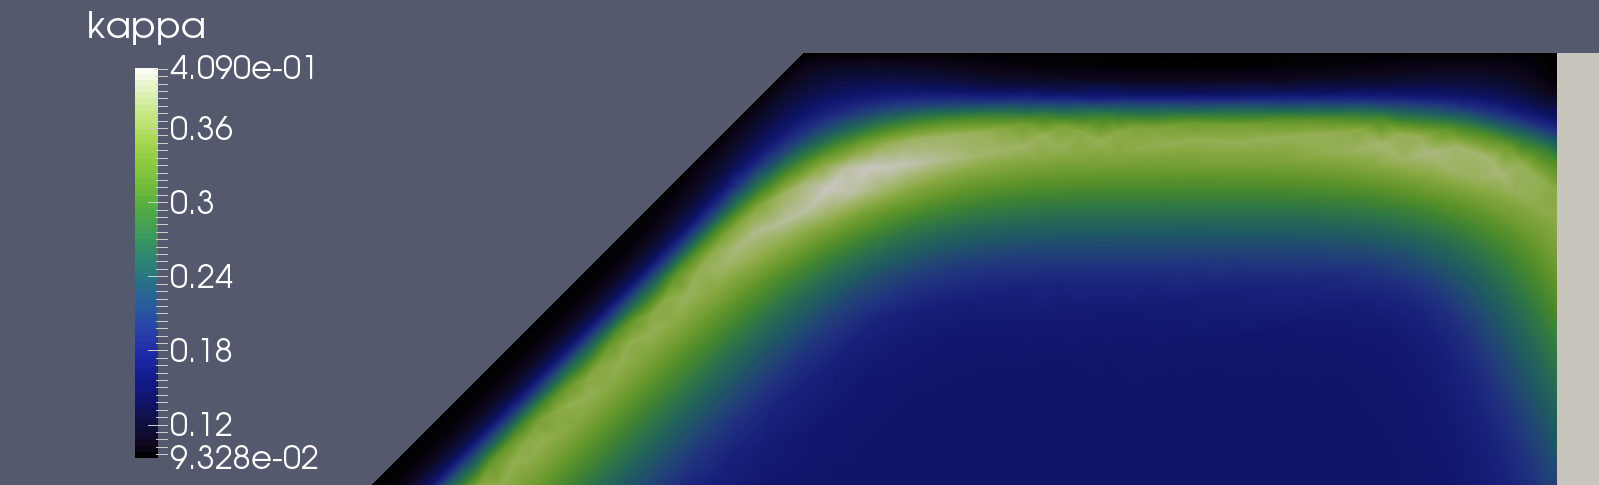
\includegraphics[width=6cm]{./Figures/smith/wall_kappa-clip.png}
%  \\[0cm]
%  \begin{itemize}
%    \setlength{\itemsep}{0.0in}
%    \item \mirgecom{} Performance \prj{\tiny}{M.~Campbell}
%      \begin{itemize}
%        \item Verification overview: testing, coverage
%        \item Performance highlights: scaling, monitoring
%      \end{itemize}
%  \end{itemize}
%  &
%  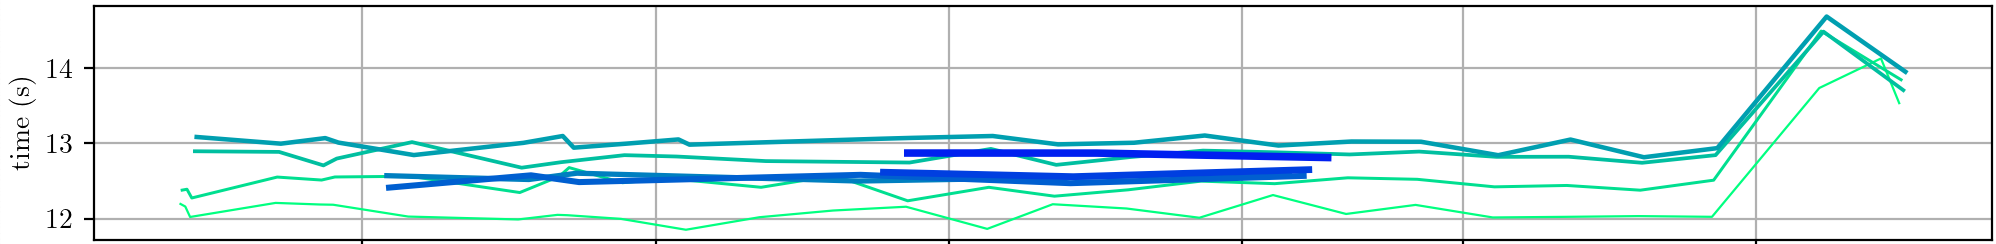
\includegraphics[width=6cm]{./Figures/timing-clip.png}
%  \\
%  \begin{itemize}
%    \setlength{\itemsep}{0.2in}
%    \item Prediction results\prj{\tiny}{M.~Anderson}
%      \begin{itemize}
%        \item Simulation status for Y3
%        \item Parsl, workflow plans \prj{\tiny}{Doug Friedel}
%      \end{itemize}
%  \end{itemize}
%  &
%  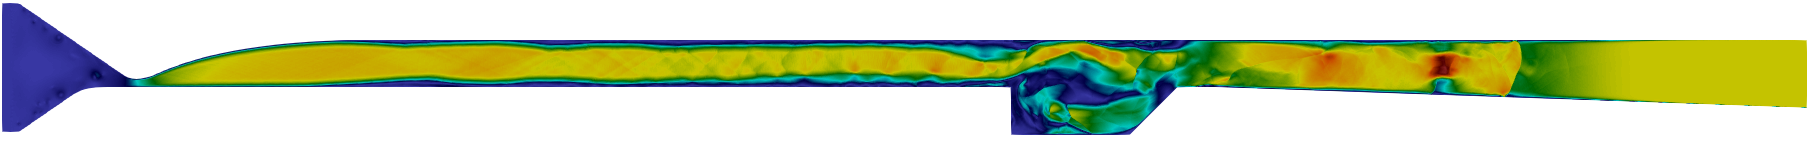
\includegraphics[width=6cm]{./Figures/Noslip_isolator_clipped.png}
%  \\
%  \begin{itemize}
%    \setlength{\itemsep}{0.2in}
%    \item Summary and risks \prj{\tiny}{Freund, Olson}
%  \end{itemize}
%  &
%  \end{tabular}
%\end{frame}
%======================================================================


\begin{frame}\frametitle{M-to-N Overview}
  \begin{itemize}
  \item What is M-to-N processing?
    \begin{itemize}
    \item Mapping of simulation data between disparate domain decompositions
    \item Required because of file-per-process I/O strategy in \mirgecom{}
    \end{itemize}
  \item What is it good for?
    \begin{itemize}
    \item Restarting \mirgecom{} on arbitrary resource size (e.g. number of GPUs)
    \item Post-processing visualization data across runs of multiple sizes
    \item Pre-partitioning reduces the memory and I/O overheads at \mirgecom{} startup
    \end{itemize}
  \end{itemize}
\end{frame}

\begin{frame}\frametitle{M-to-N Procedure Outline}
\begin{minipage}{0.49\textwidth}
\begin{itemize}
\item Generate the input mesh (\textit{gmsh} or built-in \textit{meshmode})
\item Create the target decompositions $M$,$N$
  \begin{itemize}
  \item Creates required mapping files
  \item Run \textit{meshdist} part to $M$, $N$ ranks
  \end{itemize}
\item Run \mirgecom{} on $M$ ranks
\begin{itemize}
%\item Example: Reading pre-generated mesh
\item Generates $M$ restart files per dump
\end{itemize}
\item Perform M-to-N transfer with \textit{redist}
\item Restart \mirgecom{} on $N$ ranks -or-
\item Post-processing/viz for $N$ ranks
\end{itemize}
\end{minipage}
\hfill
\begin{minipage}{.49\textwidth}
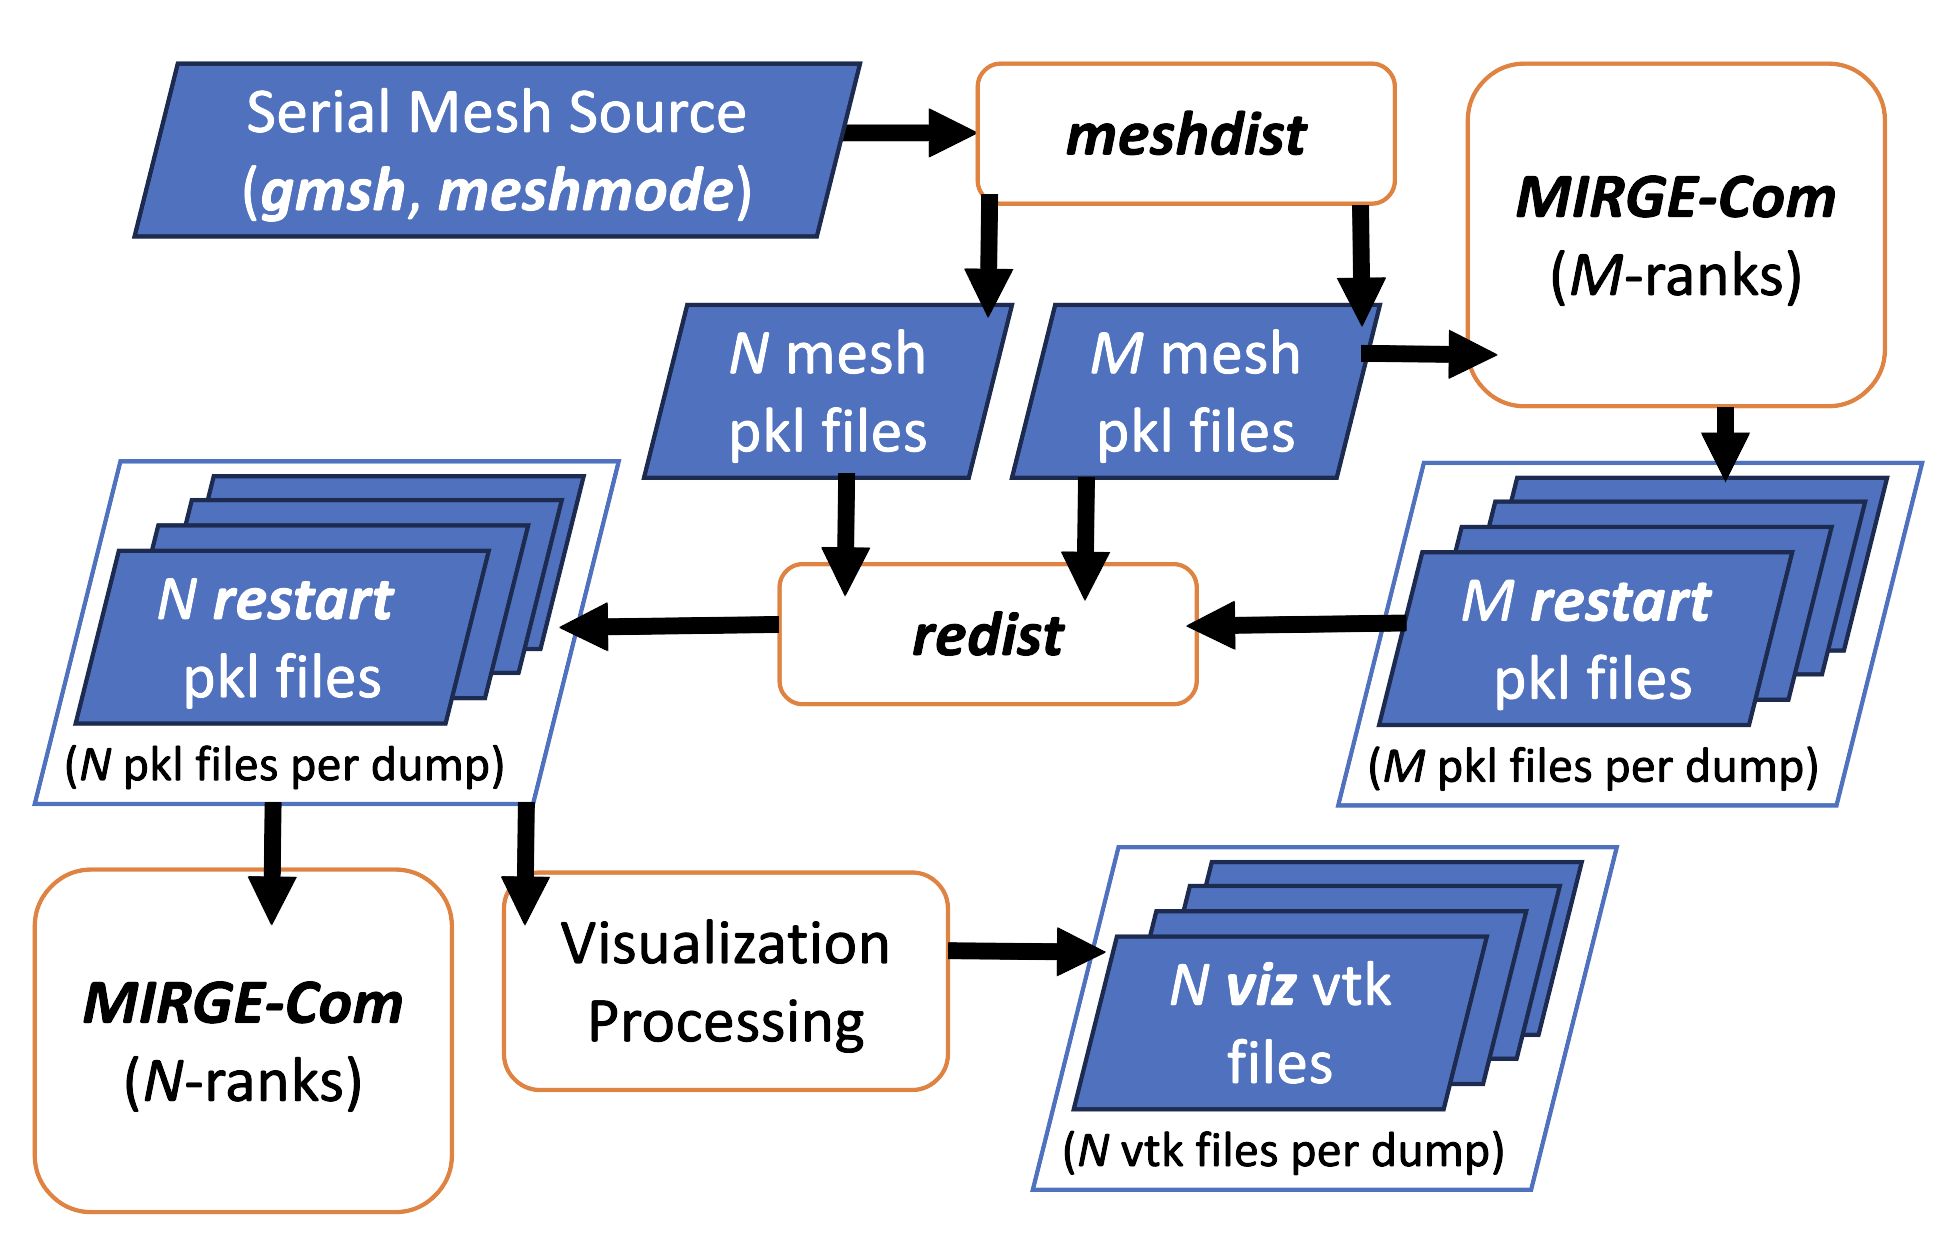
\includegraphics[width=\textwidth]{Figures/mtc/redist_data_flow_full.png}
\end{minipage}
\end{frame}

\begin{frame}\frametitle{M-to-N Procedure Outline}
\begin{minipage}{0.49\textwidth}
\begin{itemize}
\item Generate the input mesh (\textit{gmsh} or built-in \textit{meshmode})
\color{lightgray}
\item Create the target decompositions $M$,$N$
  \begin{itemize}
  \color{lightgray}
  \item Creates required mapping files
  \item Run \textit{meshdist} part to $M$, $N$ ranks
  \end{itemize}
\item Run \mirgecom{} on $M$ ranks
\begin{itemize}
\color{lightgray}
%\item Example: Reading pre-generated mesh
\item Generates $M$ restart files per dump
\end{itemize}
\item Perform M-to-N transfer with \textit{redist}
\item Restart \mirgecom{} on $N$ ranks -or-
\item Post-processing/viz for $N$ ranks
\end{itemize}
\end{minipage}
\hfill
\begin{minipage}{.49\textwidth}
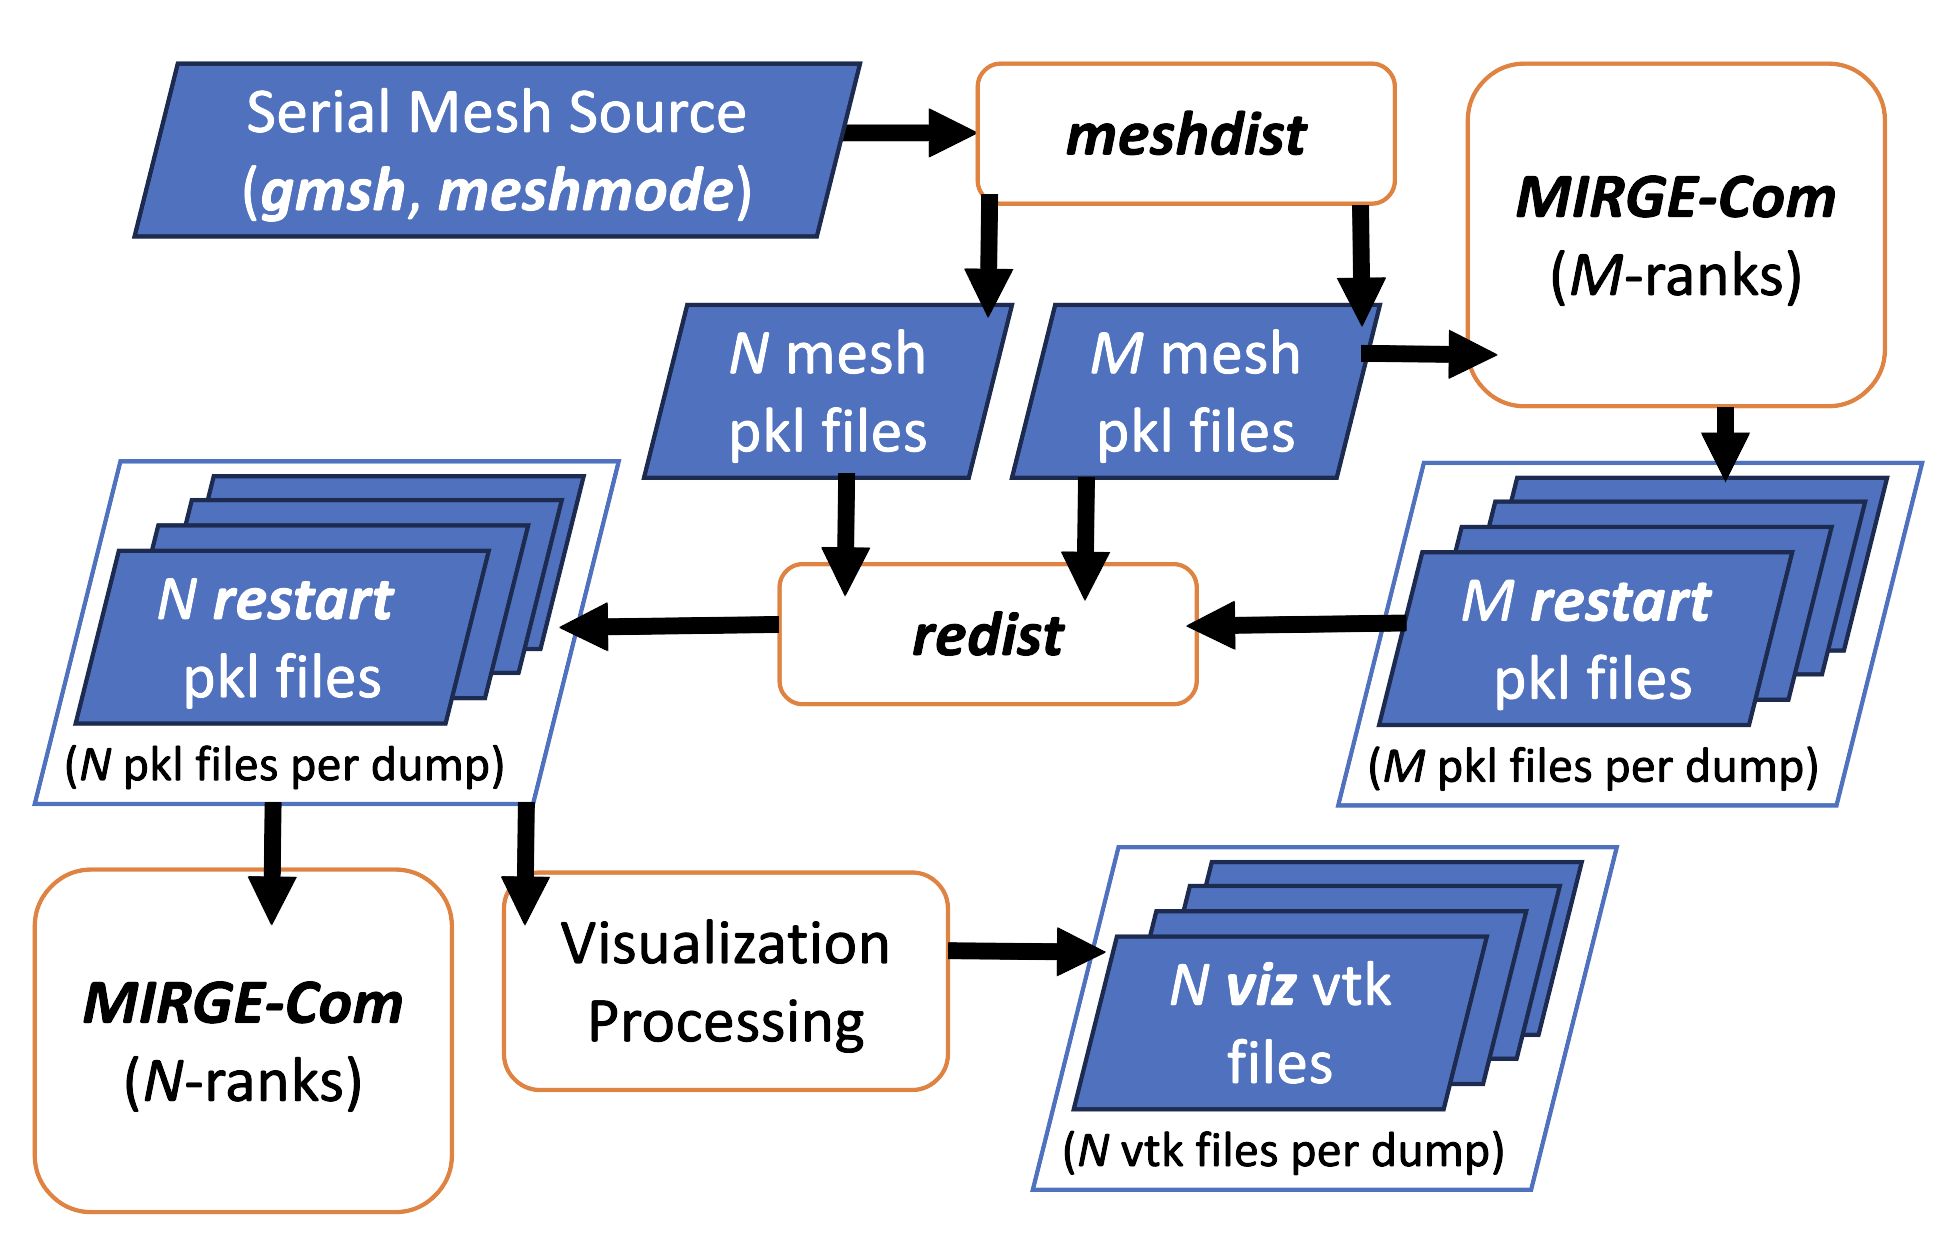
\includegraphics[width=\textwidth]{Figures/mtc/redist_data_flow_full.png}
\end{minipage}
\end{frame}


% ========= Simple examples of grid generation and import from gmsh ==============
\begin{frame}[fragile]\frametitle{Generate a Mesh with Meshmode \prj{\tiny}{M.~Smith}}

\begin{minipage}{0.5\textwidth}
\begin{itemize}
\item Mesh generator functions in \textit{meshmode} can be used to create simple
  geometries
\end{itemize}
\end{minipage}

\begin{tikzpicture}[overlay,remember picture]
\node(code)at([xshift=-1.3in,yshift=-0.5in]current page.center){
  \begin{minipage}{0.5\textwidth}
    \begin{lstlisting}[style=mintedlike,basicstyle=\mintedlikebasicstyle{\footnotesize}]
  from meshmode.mesh.generation import \
      generate_regular_rect_mesh
  mesh = generate_regular_rect_mesh(
      a=(-L/2, -L/2),
      b=(L/2, L/2),
      n=16,
      boundary_tag_to_face={
          "LeftRight": ["-x", "+x"],
          "BottomTop": ["-y", "+y"]})
    \end{lstlisting}
  \end{minipage}
};
\end{tikzpicture}
\hfill
\begin{minipage}{0.5\textwidth}

\begin{tikzpicture}[scale=0.4]
    % Grid
    \draw[step=1, thin, black] (0,0) grid (16,10);
    \draw[thick] (0,0) rectangle (16,10);
\end{tikzpicture}
\end{minipage}

\end{frame}

\begin{frame}[fragile]\frametitle{Generate Multivolume Mesh with Meshmode}

\begin{minipage}{0.5\textwidth}
\begin{itemize}
\item Creation of multi-volume mesh with \textit{meshmode}
\end{itemize}
\end{minipage}

\begin{tikzpicture}[overlay,remember picture]
\node(code)at([xshift=-1.3in,yshift=-0.5in]current page.center){
  \begin{minipage}{0.5\textwidth}
    \begin{lstlisting}[style=mintedlike,basicstyle=\mintedlikebasicstyle{\footnotesize}]
  from meshmode.mesh.generation import \
      generate_regular_rect_mesh
  mesh = generate_regular_rect_mesh(
      a=(-L/2, -L/2),
      b=(L/2, L/2),
      n=16,
      boundary_tag_to_face={
          "LeftRight": ["-x", "+x"],
          "BottomTop": ["-y", "+y"]})
  x_avg = np.sum(x, axis=1)/x.shape[1]
  tag_to_elements = {
      "Vol1": np.where(x_avg < vol1_loc)[0],
      "Vol2": np.where(x_avg > vol1_loc)[0]}
    \end{lstlisting}
  \end{minipage}
};
\end{tikzpicture}
\hfill
\begin{minipage}{0.5\textwidth}
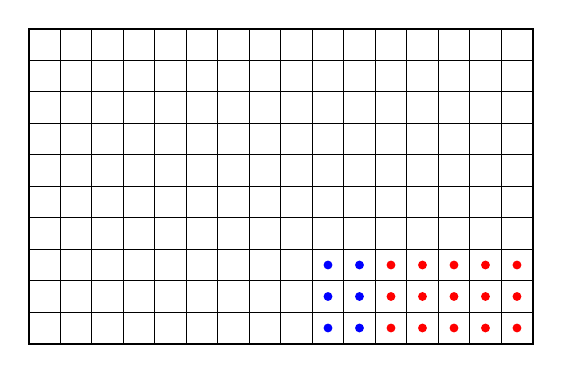
\begin{tikzpicture}[scale=0.4]
    % Grid
    \draw[step=1, thin, black] (0,0) grid (16,10);
    \draw[thick] (0,0) rectangle (16,10);
    % Red subregion
    \foreach \i in {11, 12, 13, 14, 15} {
        \foreach \j in {0, 1, 2} {
            \fill[red] (\i+0.5, \j+0.5) circle (4pt);
        }
    }
    
    % Blue subregion
    \foreach \i in {9, 10} {
        \foreach \j in {0, 1, 2} {
            \fill[blue] (\i+0.5, \j+0.5) circle (4pt);
        }
    }
\end{tikzpicture}
\begin{tikzpicture}[overlay, remember picture, scale=0.3]
  % Legend Box
  \begin{scope}[xshift=-20.8cm, yshift=16.8cm]
    \draw[thick] (-1,0.5) rectangle (6,-3);
   
    \fill[blue] (0,-0.5) circle (6pt); % Blue dot
    \node[align=left] at (3,-0.5) {Volume 1};
     
    \fill[red] (0,-2) circle (6pt);  % Red dot
    \node[align=left] at (3,-2) {Volume 2};
  \end{scope}
\end{tikzpicture}
\end{minipage}

\end{frame}


\begin{frame}[fragile]\frametitle{Generate a Tensor Product Mesh with Meshmode}

\begin{minipage}{0.5\textwidth}
\begin{itemize}
\item Creation of tensor product element mesh with \textit{meshmode}
\end{itemize}
\end{minipage}

\begin{tikzpicture}[overlay,remember picture]
\node(code)at([xshift=-1.3in,yshift=-0.5in]current page.center){
  \begin{minipage}{0.5\textwidth}
    \begin{lstlisting}[style=mintedlike,basicstyle=\mintedlikebasicstyle{\footnotesize}]
  from meshmode.mesh import \
      TensorProductElementGroup
  from meshmode.mesh.generation import \
      generate_regular_rect_mesh
  mesh = generate_regular_rect_mesh(
      a=(-L/2, -L/2),
      b=(L/2, L/2),
      n=16,
      boundary_tag_to_face={
          "LeftRight": ["-x", "+x"],
          "BottomTop": ["-y", "+y"]},
      group_cls=TensorProductElementGroup)
    \end{lstlisting}
  \end{minipage}
};
\end{tikzpicture}
\hfill
\begin{minipage}{0.5\textwidth}

\begin{tikzpicture}[scale=0.4]
    % Grid
    \draw[step=1, thin, black] (0,0) grid (16,10);
    \draw[thick] (0,0) rectangle (16,10);
\end{tikzpicture}
\end{minipage}

\end{frame}


\begin{frame}[fragile]\frametitle{Import a Gmsh Mesh \prj{\tiny}{M.~Smith}}
\vspace{-0.9in}

\begin{minipage}{0.5\textwidth}
\begin{itemize}
\item Otherwise, use \textit{Gmsh} to generate meshes from CAD
\item Multi-volume supported natively in \textit{Gmsh}
\end{itemize}
\end{minipage}

\begin{tikzpicture}[overlay,remember picture]
\node(code)at([xshift=-1.3in,yshift=-0.5in]current page.center){
  \begin{minipage}{0.5\textwidth}
    \begin{lstlisting}[style=mintedlike,basicstyle=\mintedlikebasicstyle{\footnotesize}]
def get_mesh_data():
  from meshmode.mesh.io import read_gmsh
  mesh, tag_to_elements = \
    read_gmsh(
       mesh_filename, force_ambient_dim=dim,
       return_tag_to_elements_map=True)
  volume_to_tags = {
     "fluid": ["fluid"],
     "wall":  ["wall_insert", "wall_surround"]
  }
  return mesh, tag_to_elements, volume_to_tags
  \end{lstlisting}
  \end{minipage}
};
\end{tikzpicture}

\begin{tikzpicture}[overlay,remember picture]
\node(anchor)at([xshift=1.6in]current page.center){};
\node(nozzlemesh)at([yshift=0.8in]anchor.center){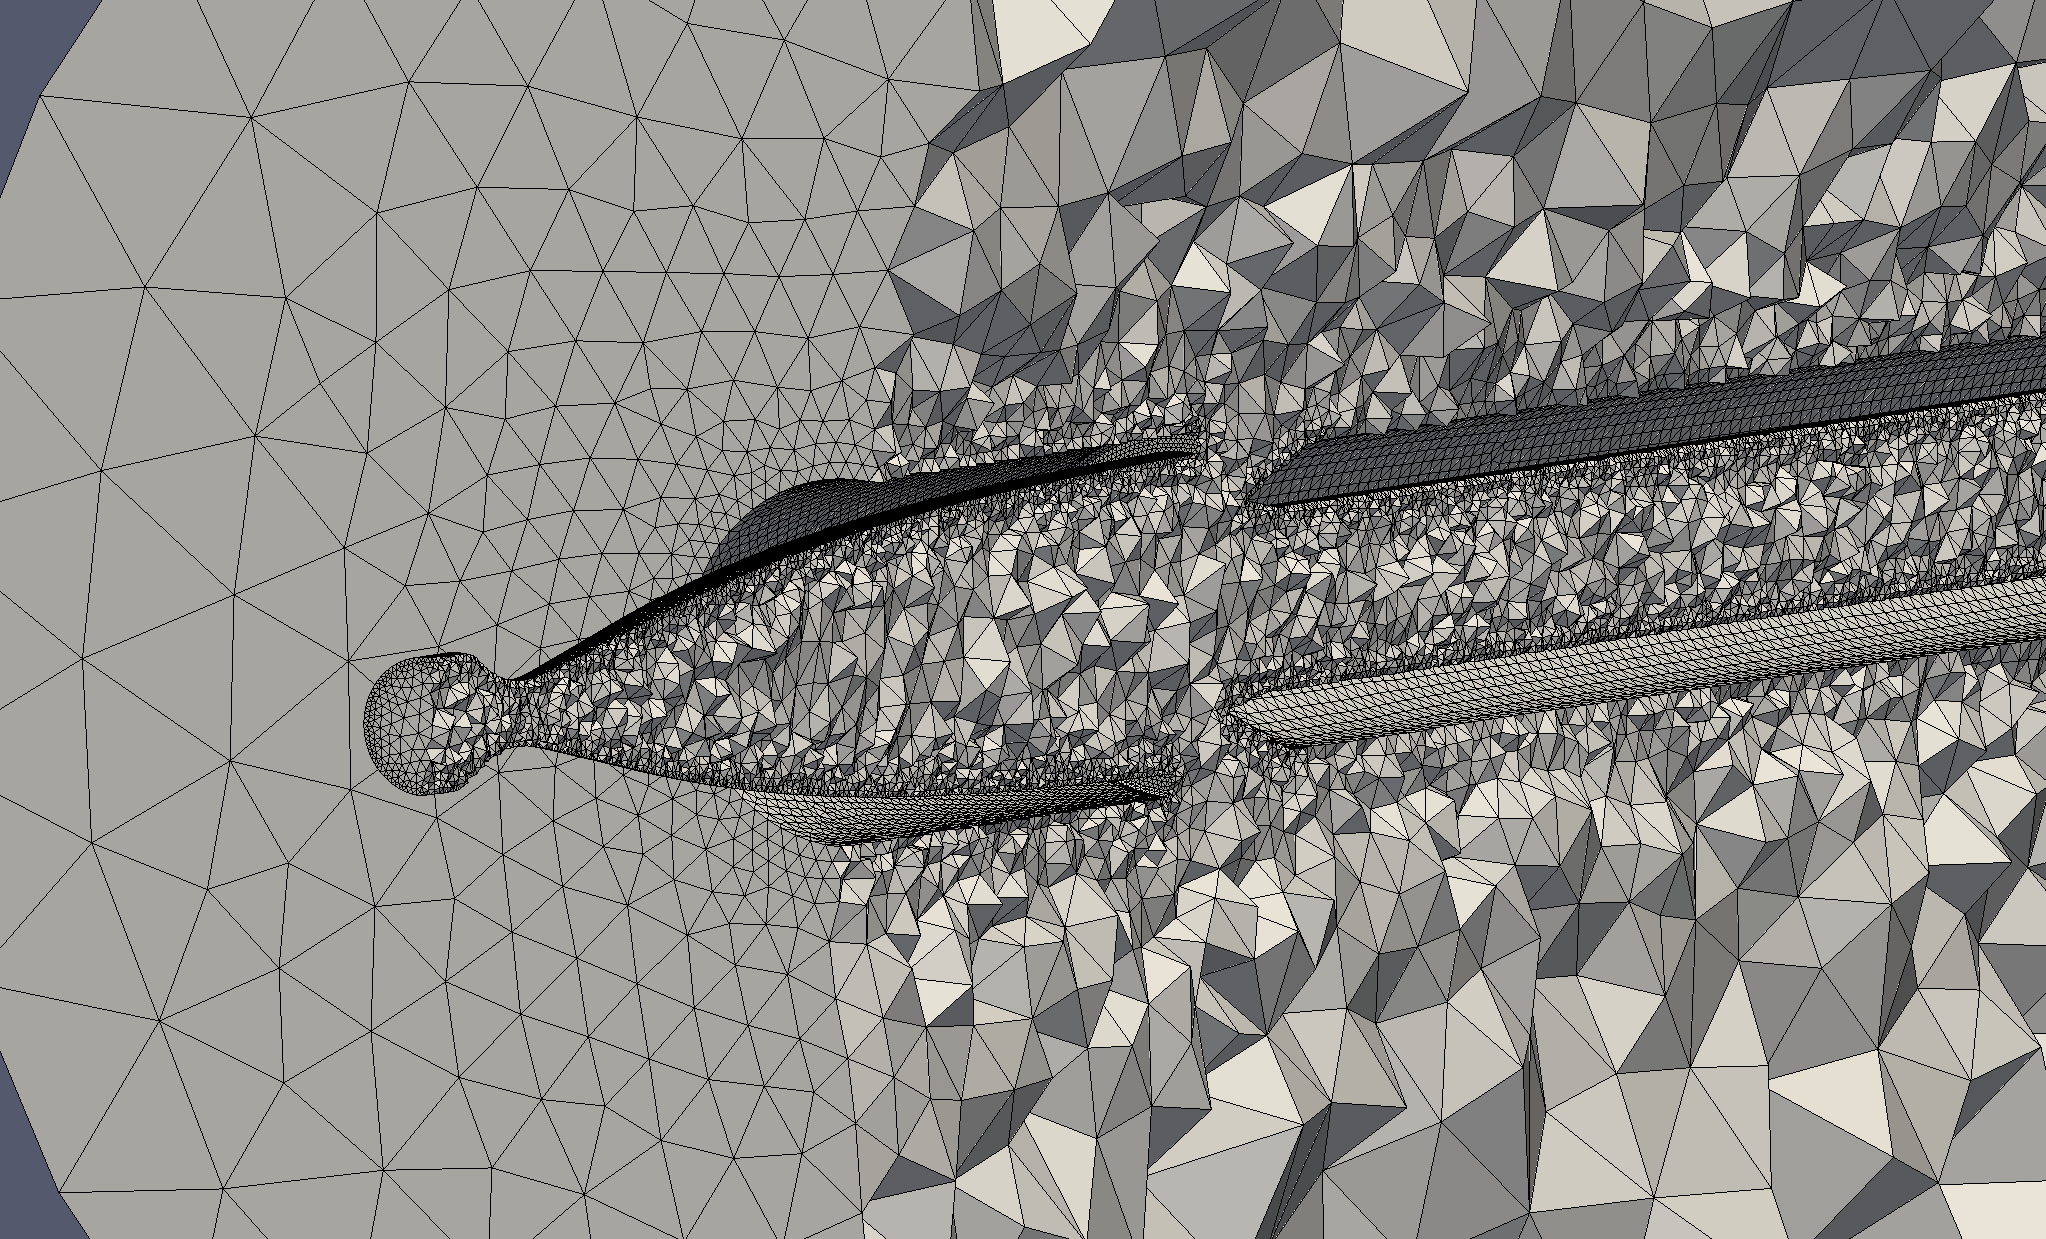
\includegraphics[width=0.4\textwidth]{Figures/mtc/nozzle_mesh.png}};
\node(y3mesh)at([yshift=-0.9in]anchor.center){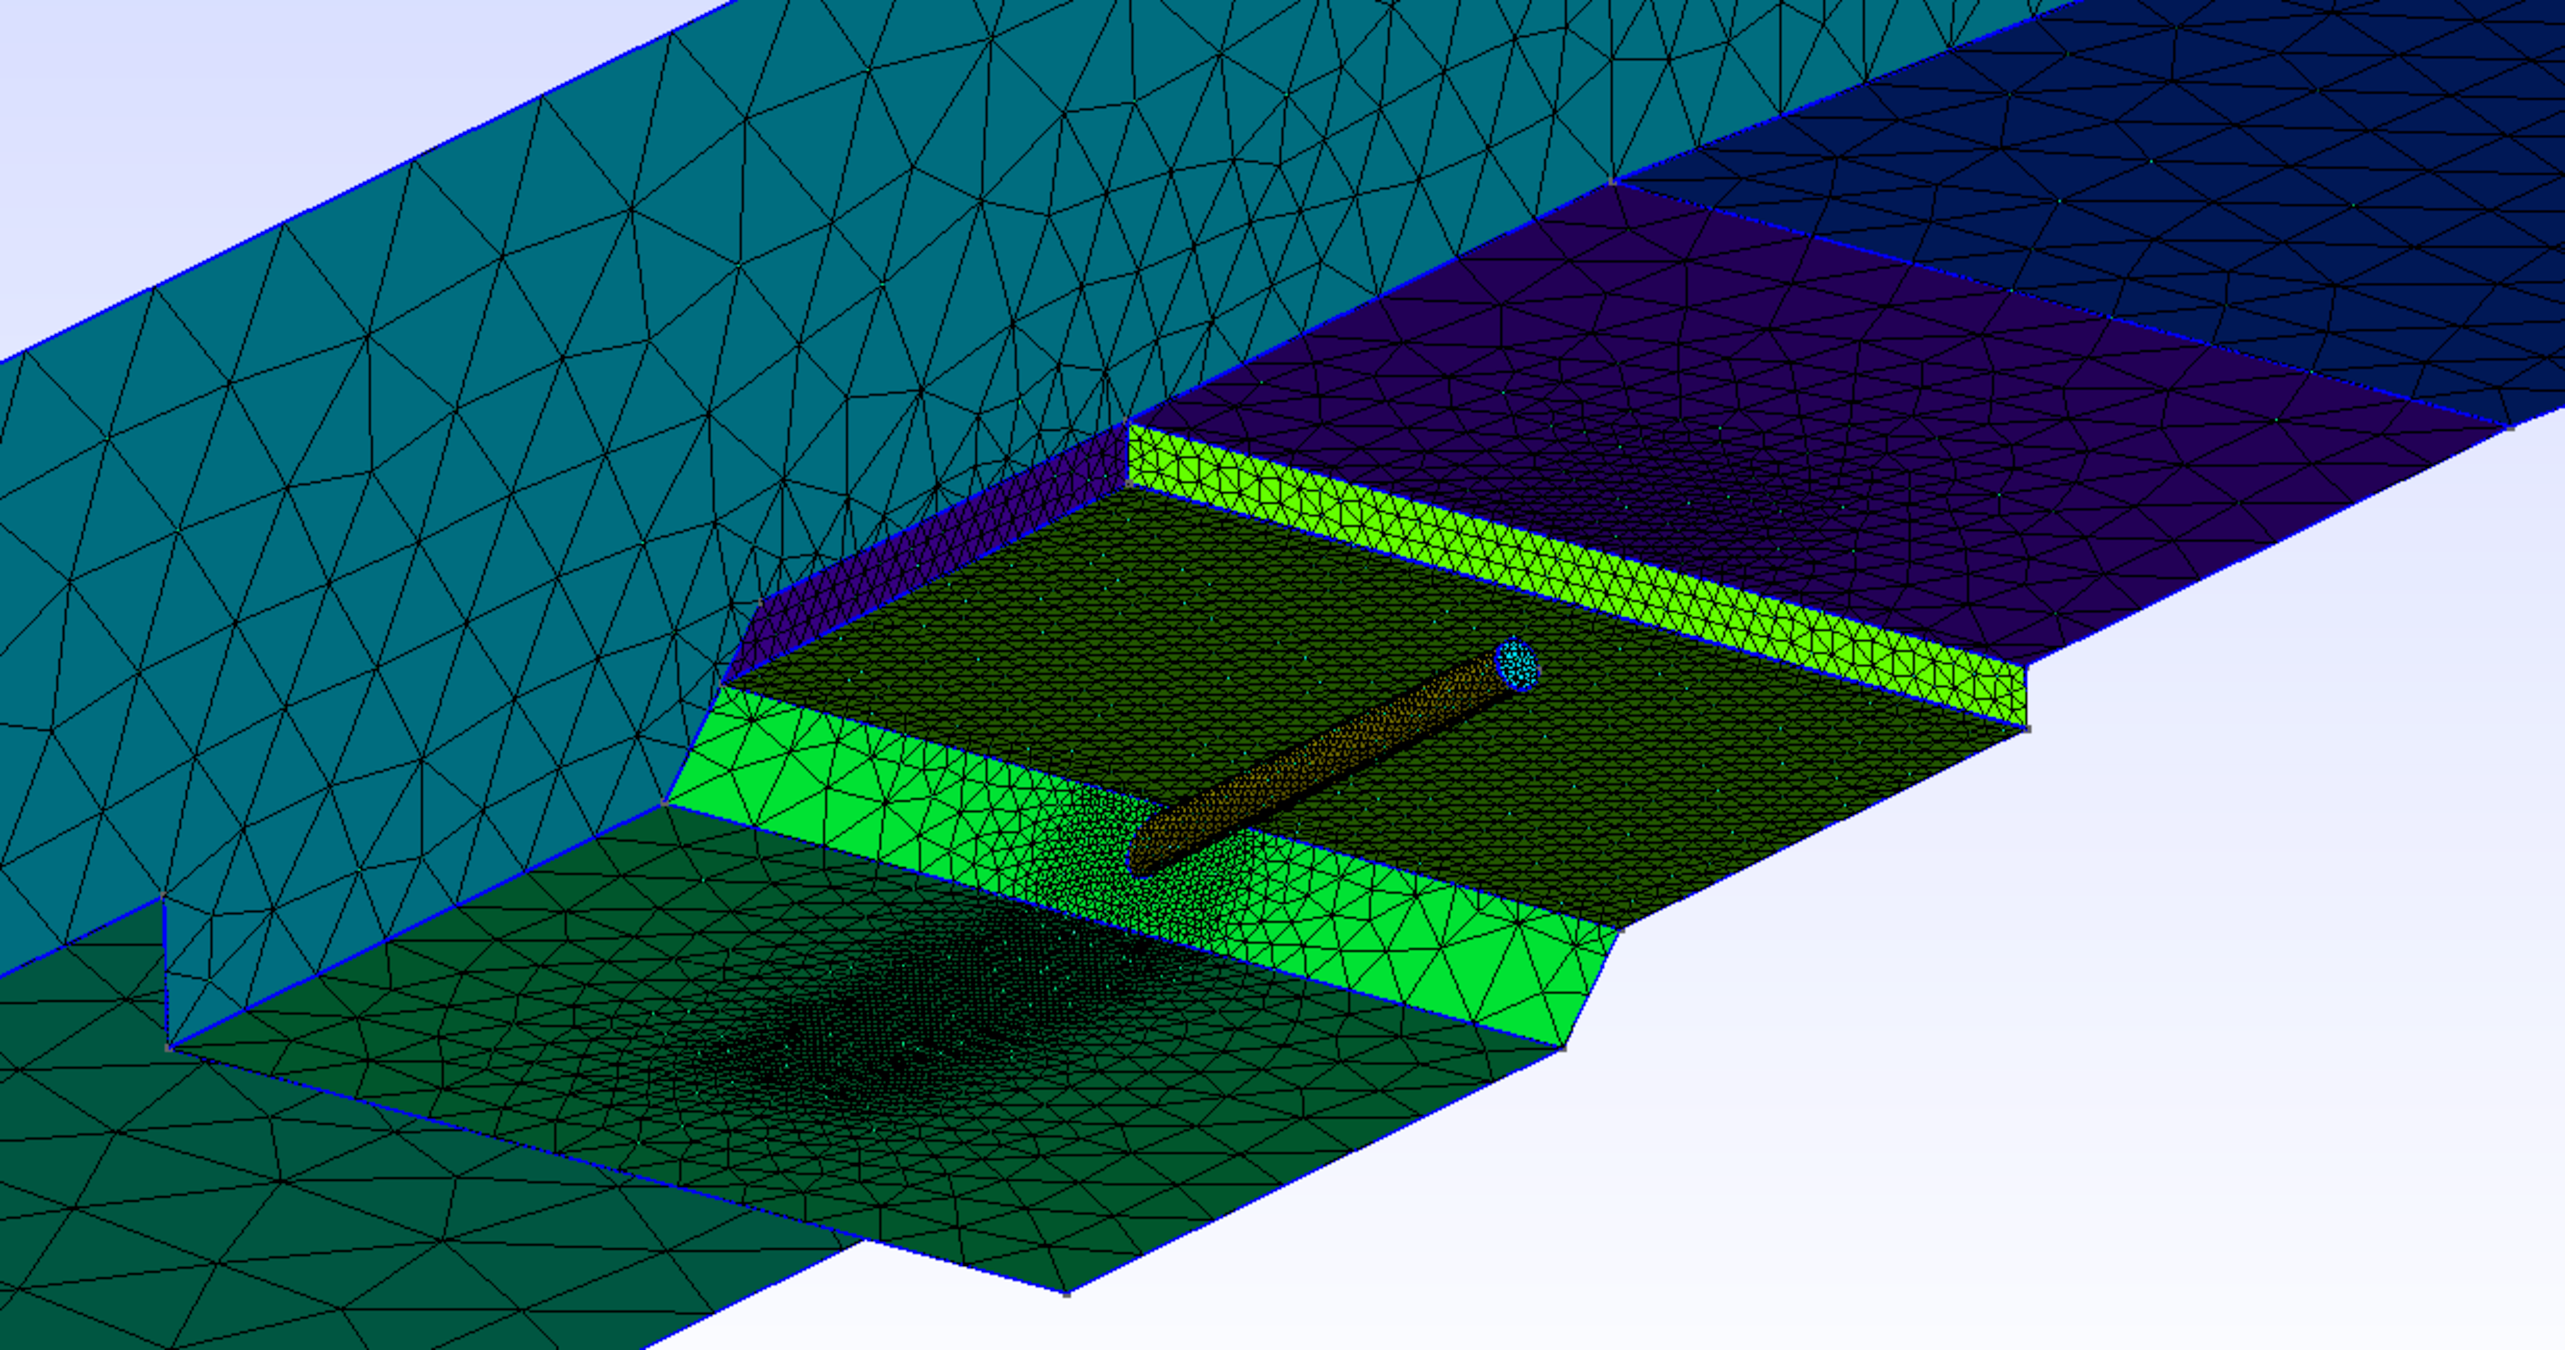
\includegraphics[width=0.4\textwidth]{Figures/mtc/3d_mesh_cavity.pdf}};
\node(ref)at([xshift=-0.1in]y3mesh.south){\prj{\tiny}{M.~Anderson, 02}};
\end{tikzpicture}

\end{frame}
% ================================================================================

% Regardless of mesh source/generator, mesh is in this general form:
\begin{frame}\frametitle{Global Mesh: Input}
\vspace{-20pt}
%\begin{minipage}[t][0.3\textheight][t]{\textwidth}
\begin{minipage}{0.5\textwidth}
\begin{itemize}
\item Gmsh, or meshmode generated mesh
  \begin{itemize}
  \item Vertex physical ($xyz$) coordinates, ($V$)
  \item Element connectivity: element-to-vertices map, ($[V][E_n]$)
  \end{itemize}
\item Total number of elements in the global mesh: $N_E$
\item Globally numbered elements: $E_n = [0, 1, 2,..., N_E)$
\item If multivolume: Tag-to-elements map, ($[E_n][tag]$)
\item Note: element numbering for unstructured mesh
\end{itemize}
\end{minipage}
\hfill
%\vfill
\begin{minipage}{0.48\textwidth}
\begin{tikzpicture}[overlay, remember picture, scale=0.4]
\begin{scope}[shift={(.5, -4)}]
    % Grid
    \draw[step=1, thin, black] (0,0) grid (16,10);
    \draw[thick] (0,0) rectangle (16,10);
    
    \def\flatteneddata{
        0, 1, 3, 6, 10, 15, 21, 28, 36, 45, 55, 65, 75, 85, 95, 105, 
        2, 4 , 7, 11, 16, 22, 29, 37, 46, 56, 66, 76, 86, 96, 106, 115, 
        5, 8, 1  2, 17, 23, 30, 38, 47, 57, 67, 77, 87, 97, 107, 116, 124, 
        9, 13, 18, 24, 31, 39, 48, 58, 68, 78, 88, 98, 108, 117, 125, 132, 
        14, 19, 25, 32, 40, 49, 59, 69, 79, 89, 99, 109, 118, 126, 133, 139, 
        20, 26, 33, 41, 50, 60, 70, 80, 90, 100, 110, 119, 127, 134, 140, 145, 
        27, 34, 42, 51, 61, 71, 81, 91, 101, 111, 120, 128, 135, 141, 146, 150, 
        35, 43, 52, 62, 72, 82, 92, 102, 112, 121, 129, 136, 142, 147, 151, 154, 
        44, 53, 63, 73, 83, 93, 103, 113, 122, 130, 137, 143, 148, 152, 155, 157, 
        54, 64, 74, 84, 94, 104, 114, 123, 131, 138, 144, 149, 153, 156, 158, 159
    }
    
    \xdef\mycount{0}
    \foreach \value in \flatteneddata {
        % Calculate x and y coordinates based on the mycount
        \pgfmathtruncatemacro\x{\mycount - 16 * (int(\mycount/16))}
        \pgfmathtruncatemacro\y{int(\mycount/16)}
        
        \node at (\x+0.5, 9.5-\y) {\tiny \value};
        
        \pgfmathtruncatemacro\incrementedcount{\mycount + 1}
        \xdef\mycount{\incrementedcount}
    }
\end{scope}
\end{tikzpicture}
\end{minipage}
\end{frame}


\begin{frame}\frametitle{M-to-N Procedure Outline}
\begin{minipage}{0.49\textwidth}
\begin{itemize}
\item {\color{lightgray}{Generate the input mesh (\textit{gmsh} or built-in \textit{meshmode}})}
\item Create the target decompositions $M$,$N$
  \begin{itemize}
  \item Creates required mapping files
  \item Run \textit{meshdist} part to $M$, $N$ ranks
  \end{itemize}
\color{lightgray}
\item Run \mirgecom{} on $M$ ranks
\begin{itemize}
\color{lightgray}
%\item Example: Reading pre-generated mesh
\item Generates $M$ restart files per dump
\end{itemize}
\item Perform M-to-N transfer with \textit{redist}
\item Restart \mirgecom{} on $N$ ranks -or-
\item Post-processing/viz for $N$ ranks
\end{itemize}
\end{minipage}
\hfill
\begin{minipage}{.49\textwidth}
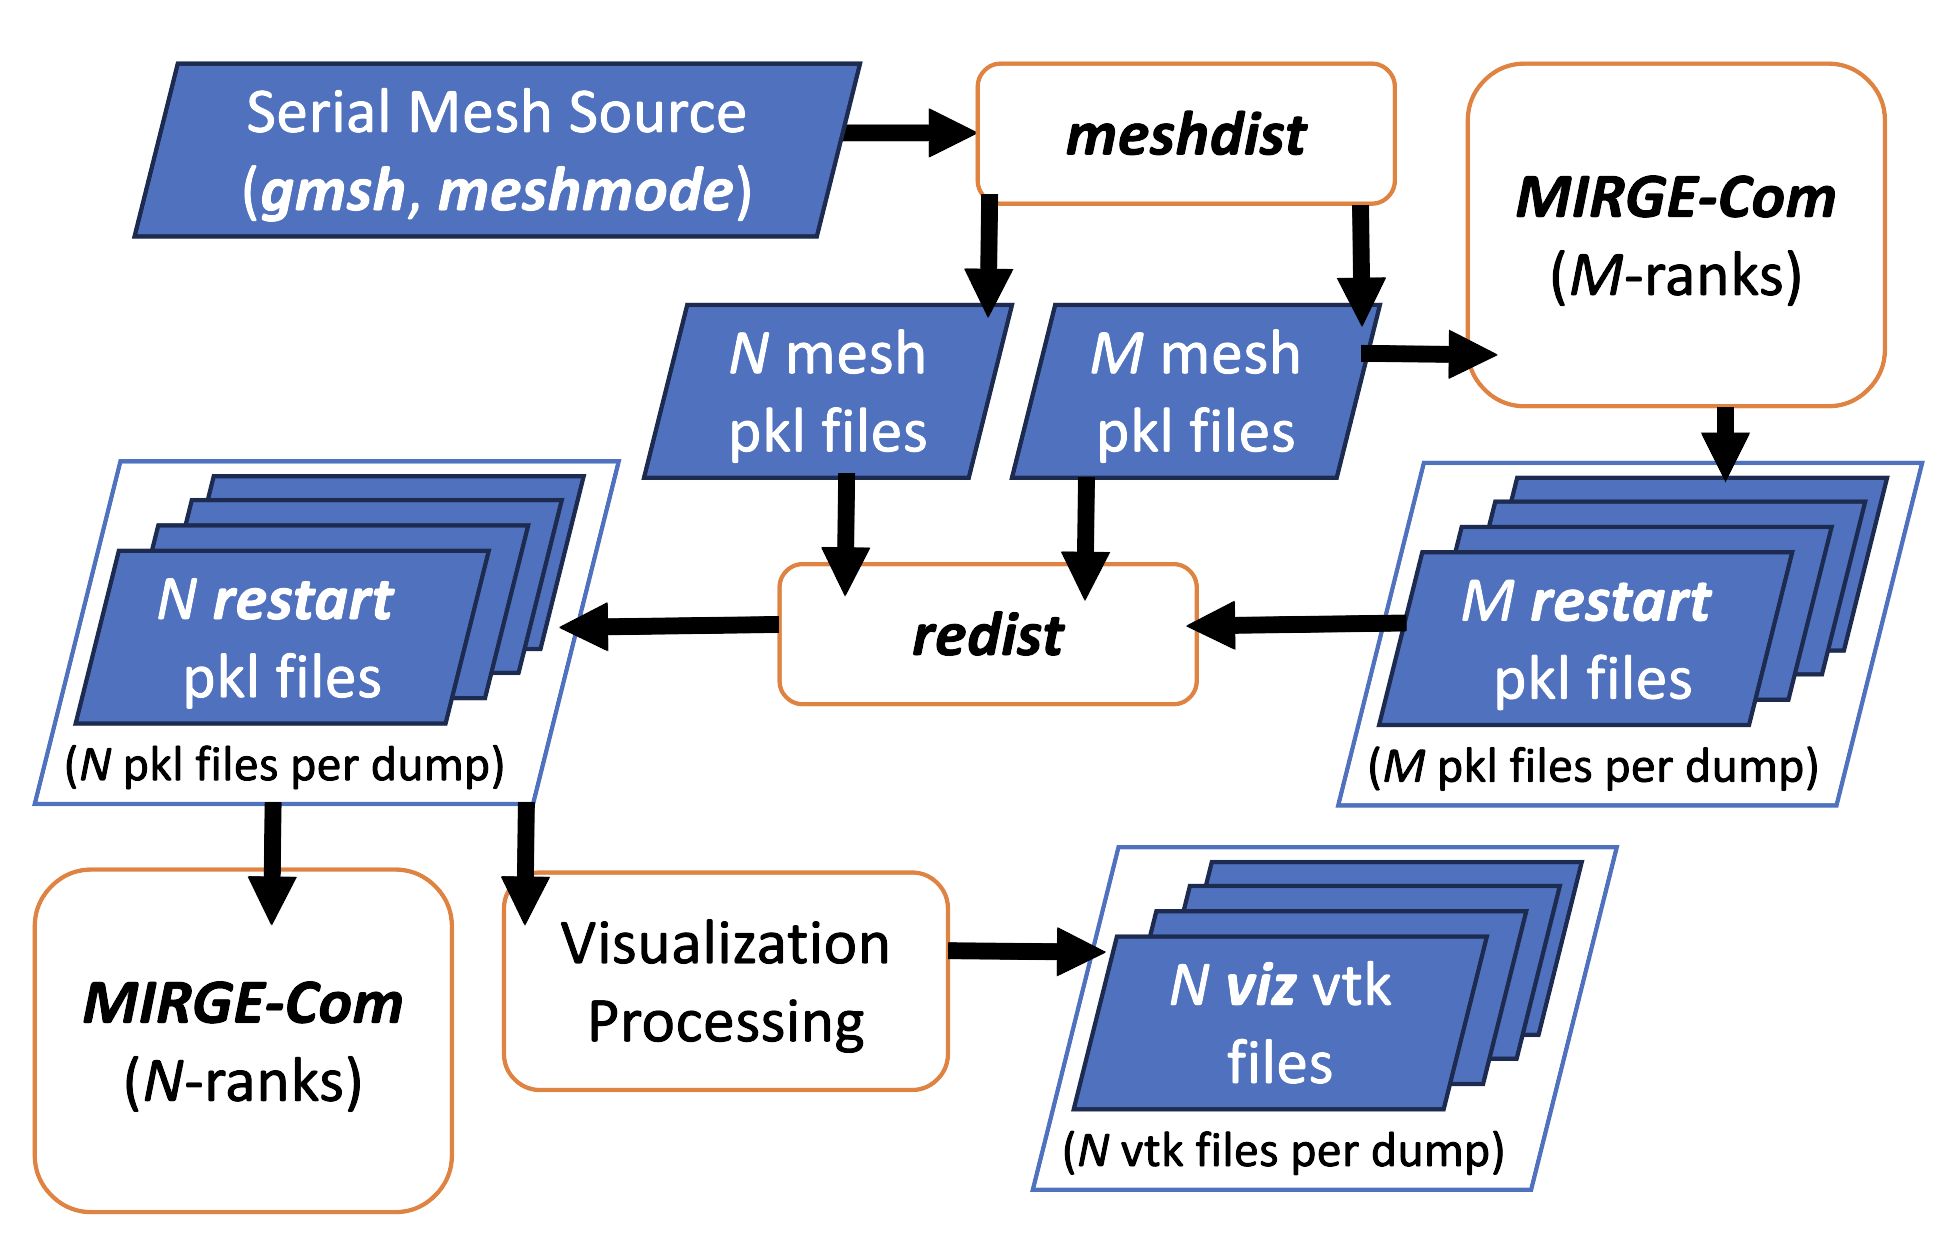
\includegraphics[width=\textwidth]{Figures/mtc/redist_data_flow_full.png}
\end{minipage}
\end{frame}

\begin{frame}\frametitle{\textit{meshdist}: \mirgecom{} Mesh Partitioning Utility}
  \begin{minipage}[t][.4\textheight][t]{\textwidth}
    \begin{multicols}{2}
      \begin{itemize}
      \item Creates $M$-decomposition of input mesh
      \item \textit{Metis} by default, 1dpart optional
      \item Mirrors built-in decomposition, \textbf{\textit{except}}:
        %\begin{itemize}
        %\item Writes mapping files required by m-to-n
          \begin{itemize}
          \item Writes decomp map: $r_m[E_N]$  (maps global element id $E_n$ to MPI rank $r_m$)
          %\item PartID map: $P[E_N]$ (maps global element id to PartID $P$)
          %\item PartID is (volume, rank) pair
          \item Writes $M$-decomposed mesh into pkl file per rank
          \end{itemize}
        %\end{itemize}
      \item Divides work across $P$ processors (max used $= M$)
        \begin{itemize}
        \item Each \textit{meshdist} rank locally handles $M/P$ mesh partitions
        \item Reads and partition input mesh on all ranks
        % \item Local meshmode datastructures for locally-handled $M$-parts
        \item Writes only locally-handled $M$-parts to pkl
        \end{itemize}
      \end{itemize}
    \end{multicols}
  \end{minipage}
  \vfill
  \center{\texttt{python -m mpi4py meshdist.py -1 -n 4 -i box.msh -o box\_4p}}
  \begin{minipage}[b][.4\textheight][t]{\textwidth}
    \begin{tikzpicture}[overlay, remember picture, scale=0.3]
      \node at (2cm, -14.5cm) (center) {};

      %\begin{scope}[shift={(center)}]  % yshift=-10cm]
      \begin{scope}[yshift=-12cm]

        % Grid
        \draw[step=1, thin, black] (0,0) grid (16,10);
        \draw[thick] (0,0) rectangle (16,10);

        \begin{scope}[xshift=30cm]
          % Partition 0
          \draw[step=1, thin, black] (0,0) grid (4,10);
          \draw[thick] (0,0) rectangle (4,10);
          \node[font=\bfseries, blue] at (2,9) {0};
    
          % Partition 1
          \begin{scope}[xshift=4.5cm]
            \draw[step=1, thin, black] (0,0) grid (4,10);
            \draw[thick] (0,0) rectangle (4,10);
            \node[font=\bfseries, blue] at (2,9) {1};
          \end{scope}
    
          % Partition 2 
          \begin{scope}[xshift=9cm]
            \draw[step=1, thin, black] (0,0) grid (4,10);
            \draw[thick] (0,0) rectangle (4,10);
            \node[font=\bfseries, blue] at (2,9) {2};
          \end{scope}
    
          % Partition 3 
          \begin{scope}[xshift=13.5cm]
            \draw[step=1, thin, black] (0,0) grid (4,10);
            \draw[thick] (0,0) rectangle (4,10);
            \node[font=\bfseries, blue] at (2,9) {3};
          \end{scope}
        \end{scope}
    
        % Coordinates for arrow
        \coordinate (leftGridCenter) at (8,5);
        \coordinate (rightGridCenter) at (38,5);
    
        % Arrow with text
        \draw[->, ultra thick] (leftGridCenter) -- node[midway, fill=white, text width=3cm, align=center] {\textit{meshdist}} (rightGridCenter);
      \end{scope}
    \end{tikzpicture}
  \end{minipage}
\end{frame}


\begin{frame}\frametitle{Multivolume Mesh with \textit{meshdist}}
  \begin{minipage}[t][.2\textheight][t]{\textwidth}
    %\begin{multicols}{2}
      \begin{itemize}
      %\item Creates $M$-decomposition of multivolume input mesh
      \item Additional data for multivolume meshes: 
          \begin{itemize}
          \item Writes PartID map: $P[E_N]$ (maps global element id to PartID $P$)
          \item PartID is (volume, rank) pair
          \end{itemize}
        %\end{itemize}
      %\item Divides work across $P$ processors (max used $= M$)
        %\begin{itemize}
        %\item Each \textit{meshdist} rank locally handles $M/P$ mesh partitions
        %\item Reads and partition input mesh on all ranks
        % \item Local meshmode datastructures for locally-handled $M$-parts
        %\item Writes only locally-handled $M$-parts to pkl
        %\end{itemize}
      \end{itemize}
    %\end{multicols}
  \end{minipage}
  \vfill
  \center{\texttt{mpiexec -n NP python -m mpi4py meshdist.py -w -1 -n 4 -i multivol.msh -o multivol\_4p}}
  \begin{minipage}[b][.4\textheight][t]{\textwidth}
    \begin{tikzpicture}[overlay, remember picture, scale=0.3]
      \begin{scope}[yshift=-12cm]
        % Grid
        \draw[step=1, thin, black] (0,0) grid (16,10);
        \draw[thick] (0,0) rectangle (16,10);
    
        % Red subregion
        \foreach \i in {11, 12, 13, 14, 15} {
          \foreach \j in {0, 1, 2} {
            \fill[red] (\i+0.5, \j+0.5) circle (4pt);
          }
        }
    
        % Blue subregion
        \foreach \i in {9, 10} {
          \foreach \j in {0, 1, 2} {
            \fill[blue] (\i+0.5, \j+0.5) circle (4pt);
          }
        }
        \begin{scope}[xshift=30cm]
          % Partition 0
          \draw[step=1, thin, black] (0,0) grid (4,10);
          \draw[thick] (0,0) rectangle (4,10);
          \node[font=\bfseries, blue] at (2,9) {0};
    
          % Partition 1
          \begin{scope}[xshift=4.5cm]
            \draw[step=1, thin, black] (0,0) grid (4,10);
            \draw[thick] (0,0) rectangle (4,10);
            \node[font=\bfseries, blue] at (2,9) {1};
          \end{scope}
    
          % Partition 2 with blue and red subregions
          \begin{scope}[xshift=9cm]
            \draw[step=1, thin, black] (0,0) grid (4,10);
            \draw[thick] (0,0) rectangle (4,10);
            \foreach \j in {0, 1, 2} {
              \fill[blue] (1.5, \j+0.5) circle (4pt);
              \fill[blue] (2.5, \j+0.5) circle (4pt);
              \fill[red] (3.5, \j+0.5) circle (4pt);
            }
            \node[font=\bfseries, blue] at (2,9) {2};
          \end{scope}
    
          % Partition 3 with red subregion
          \begin{scope}[xshift=13.5cm]
            \draw[step=1, thin, black] (0,0) grid (4,10);
            \draw[thick] (0,0) rectangle (4,10);
            \foreach \j in {0, 1, 2} {
              \fill[red] (0.5, \j+0.5) circle (4pt);
              \fill[red] (1.5, \j+0.5) circle (4pt);
              \fill[red] (2.5, \j+0.5) circle (4pt);
              \fill[red] (3.5, \j+0.5) circle (4pt);
            }
            \node[font=\bfseries, blue] at (2,9) {3};
          \end{scope}
        \end{scope}
        % Coordinates for arrow
        \coordinate (leftGridCenter) at (8,5);
        \coordinate (rightGridCenter) at (38,5);
        
        % Arrow with text
        \draw[->, ultra thick] (leftGridCenter) -- node[midway, fill=white, text width=3cm, align=center] {\textit{meshdist}} (rightGridCenter);
      \end{scope}
    \end{tikzpicture}
  \end{minipage}
\end{frame}

\begin{frame}\frametitle{M-to-N Procedure Outline}
\begin{minipage}{0.49\textwidth}
\begin{itemize}
\item {\color{lightgray}{Generate the input mesh (\textit{gmsh} or built-in \textit{meshmode}})}
\item {\color{lightgray}{Create the target decompositions $M$,$N$}}
  \begin{itemize}
  \color{lightgray}
  \item Creates required mapping files
  \item Run \textit{meshdist} part to $M$, $N$ ranks
  \end{itemize}
\item Run \mirgecom{} on $M$ ranks
\begin{itemize}
%\item Example: Reading pre-generated mesh
\item Generates $M$ restart files per dump
\end{itemize}
\color{lightgray}
\item Perform M-to-N transfer with \textit{redist}
\item Restart \mirgecom{} on $N$ ranks -or-
\item Post-processing/viz for $N$ ranks
\end{itemize}
\end{minipage}
\hfill
\begin{minipage}{.49\textwidth}
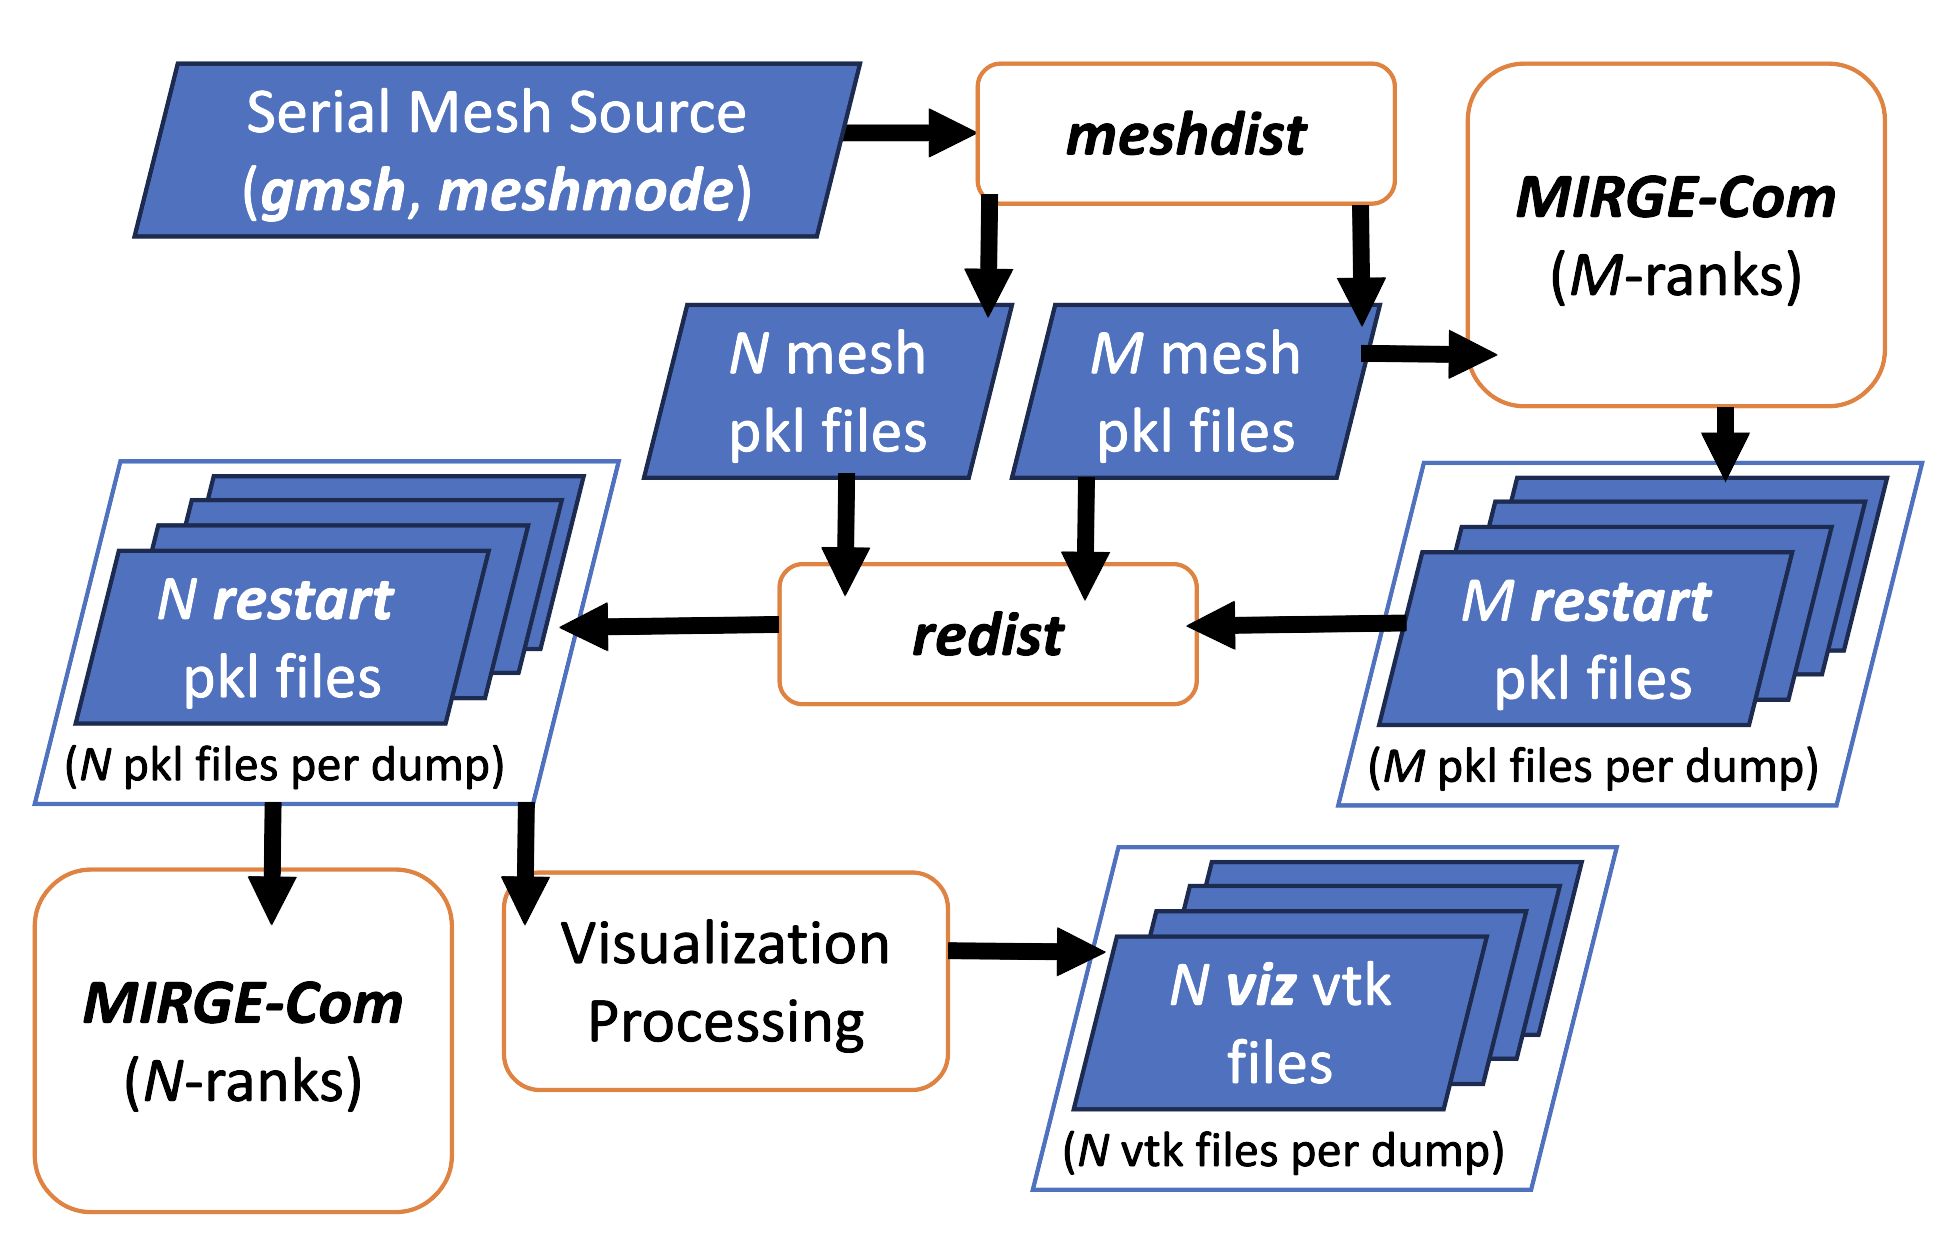
\includegraphics[width=\textwidth]{Figures/mtc/redist_data_flow_full.png}
\end{minipage}
\end{frame}

\begin{frame}\frametitle{Run \mirgecom{} on $M$ MPI Ranks (Multivolume)}
   \begin{minipage}[t][.4\textheight][t]{\textwidth}
    %\begin{multicols}{2}
      \begin{itemize}
      \item Reads $M$-partitioned input mesh
      \item Initializes \textit{volume-specific} solution
      \item Each solution dump is 1 PKL file per MPI rank with:
        \begin{itemize}
        \item Volume-specific DOFArray sizes correspond to PartIDs
        \item Arbitrary data structures in I/O dictionary 
        \end{itemize}
      \end{itemize}
    %\end{multicols}
  \end{minipage}
  \vfill
  \center{\texttt{mpiexec -n 4 python -m mpi4py prediction.py -i run\_params.yaml --lazy}}
  \begin{minipage}[b][.4\textheight][t]{\textwidth}
    \begin{tikzpicture}[overlay, remember picture, scale=0.25]
      \node at (2cm, -14.5cm) (center) {};

      %\begin{scope}[shift={(center)}]  % yshift=-10cm]
      \begin{scope}[yshift=-12cm]
        % Partition 0
        \draw[step=1, thin, black] (0,0) grid (4,10);
        \draw[thick] (0,0) rectangle (4,10);
        \node[font=\bfseries, blue] at (2,9) {0};
        
        % Partition 1
        \begin{scope}[xshift=4.5cm]
          \draw[step=1, thin, black] (0,0) grid (4,10);
          \draw[thick] (0,0) rectangle (4,10);
          \node[font=\bfseries, blue] at (2,9) {1};
        \end{scope}
    
        % Partition 2 with blue and red subregions
        \begin{scope}[xshift=9cm]
          \draw[step=1, thin, black] (0,0) grid (4,10);
          \draw[thick] (0,0) rectangle (4,10);
          \foreach \j in {0, 1, 2} {
            \fill[blue] (1.5, \j+0.5) circle (4pt);
            \fill[blue] (2.5, \j+0.5) circle (4pt);
            \fill[red] (3.5, \j+0.5) circle (4pt);
          }
          \node[font=\bfseries, blue] at (2,9) {2};
        \end{scope}
    
        % Partition 3 with red subregion
        \begin{scope}[xshift=13.5cm]
          \draw[step=1, thin, black] (0,0) grid (4,10);
          \draw[thick] (0,0) rectangle (4,10);
          \foreach \j in {0, 1, 2} {
            \fill[red] (0.5, \j+0.5) circle (4pt);
            \fill[red] (1.5, \j+0.5) circle (4pt);
            \fill[red] (2.5, \j+0.5) circle (4pt);
            \fill[red] (3.5, \j+0.5) circle (4pt);
          }
          \node[font=\bfseries, blue] at (2,9) {3};
        \end{scope}
        \begin{scope}[xshift=40cm]
          % Partition (0,0)
          \draw[step=1, thin, black] (0,0) grid (4,10);
          \draw[thick] (0,0) rectangle (4,10);
          \node[font=\bfseries, blue] at (2,9) {(0,0)};

          % Partition (1,0)
          \begin{scope}[xshift=4.5cm]
            \draw[step=1, thin, black] (0,0) grid (4,10);
            \draw[thick] (0,0) rectangle (4,10);
            \node[font=\bfseries, blue] at (2,9) {(1,0)};
          \end{scope}

          % Partition (2,0) 
          \begin{scope}[xshift=9cm]
            \foreach \i in {0,1,2,3} {
              \foreach \j in {3,4,...,9} {
                \draw (\i,\j) rectangle (\i+1,\j+1);
              }
            }
            \draw (0,0) rectangle (1,3);
            \draw (0,0) rectangle (1,1);
            \draw (0,1) rectangle (1,2);
            \draw (0,2) rectangle (1,3);
            \draw[thick] (0,0) -- (1,0) -- (1,3) -- (4,3) -- (4,10) -- (0,10) -- cycle;
            \node[font=\bfseries, blue] at (2,9) {(2,0)};
          \end{scope}

          % Partition (2,1) with blue subregion
          \begin{scope}[xshift=13.5cm, yshift=6cm]
            \draw[step=1, thin, black] (0,0) grid (2,4);
            \draw[thick] (0,0) rectangle (2,4);
            \foreach \j in {0,1,2,3} {
              \fill[blue] (0.5, \j+0.5) circle (4pt);
              \fill[blue] (1.5, \j+0.5) circle (4pt);
            }
            \node[font=\bfseries, blue] at (1,3) {(2,1)};
          \end{scope}

          % Partition (2,2) with red subregion
          \begin{scope}[xshift=13.5cm, yshift=2cm]
            \draw[step=1, thin, black] (0,0) grid (1,3);
            \draw[thick] (0,0) rectangle (1,3);
            \foreach \j in {0,1,2} {
              \fill[red] (0.5, \j+0.5) circle (4pt);
            }
            \node[font=\bfseries, blue] at (0.5,2) {(2,2)};
          \end{scope}

          % Partition (3,0)
          \begin{scope}[xshift=16cm, yshift=3.5cm]
            \draw[step=1, thin, black] (0,0) grid (4,7);
            \draw[thick] (0,0) rectangle (4,7);
            \node[font=\bfseries, blue] at (2,6) {(3,0)};
          \end{scope}

          % Partition (3,2) with red subregion
          \begin{scope}[xshift=16cm, yshift=-0.5cm]
            \draw[step=1, thin, black] (0,0) grid (4,3);
            \draw[thick] (0,0) rectangle (4,3);
            \foreach \j in {0,1,2} {
              \fill[red] (0.5, \j+0.5) circle (4pt);
              \fill[red] (1.5, \j+0.5) circle (4pt);
              \fill[red] (2.5, \j+0.5) circle (4pt);
              \fill[red] (3.5, \j+0.5) circle (4pt);
            }
            \node[font=\bfseries, blue] at (2,2) {(3,2)};
          \end{scope}
        \end{scope}
        \begin{scope}[xshift=5cm]
          % Coordinates for arrow
          \coordinate (leftGridCenter) at (8,5);
          \coordinate (rightGridCenter) at (38,5);
        
          % Arrow with text
          \draw[->, ultra thick] (leftGridCenter) -- node[midway, fill=white, text width=3cm, align=center] {\textit{MIRGE-Com}} (rightGridCenter);
        \end{scope}
      \end{scope}
    \end{tikzpicture}
  \end{minipage}
\end{frame}

\begin{frame}\frametitle{\mirgecom{} I/O Datastructure}
  \begin{itemize}
  \item Arbitrary, user-defined I/O data from \mirgecom{}
  \item No reliable way to associate DOFArrays with PartIDs
  \item Really convenient; almost completely bonkers
  \end{itemize}
\begin{tikzpicture}
  \node at (0,0) {\snippetboxbigtab{Figures/mtc/write_restart.py}{\href{https://github.com/illinois-ceesd/drivers_y3-prediction/blob/main/y3prediction/prediction.py}{prediction\_write\_restart}}};
\end{tikzpicture}
\end{frame}

\begin{frame}\frametitle{M-to-N Procedure Outline}
\begin{minipage}{0.49\textwidth}
\begin{itemize}
\item {\color{lightgray}{Generate the input mesh (\textit{gmsh} or built-in \textit{meshmode}})}
\item {\color{lightgray}{Create the target decompositions $M$,$N$}}
  \begin{itemize}
  \color{lightgray}
  \item Creates required mapping files
  \item Run \textit{meshdist} part to $M$, $N$ ranks
  \end{itemize}
\item {\color{lightgray}{Run \mirgecom{} on $M$ ranks}}
  \begin{itemize}
    \color{lightgray}
    %\item Example: Reading pre-generated mesh
  \item Generates $M$ restart files per dump
  \end{itemize}
\item Perform M-to-N transfer with \textit{redist}
\color{lightgray}
\item Restart \mirgecom{} on $N$ ranks -or-
\item Post-processing/viz for $N$ ranks
\end{itemize}
\end{minipage}
\hfill
\begin{minipage}{.49\textwidth}
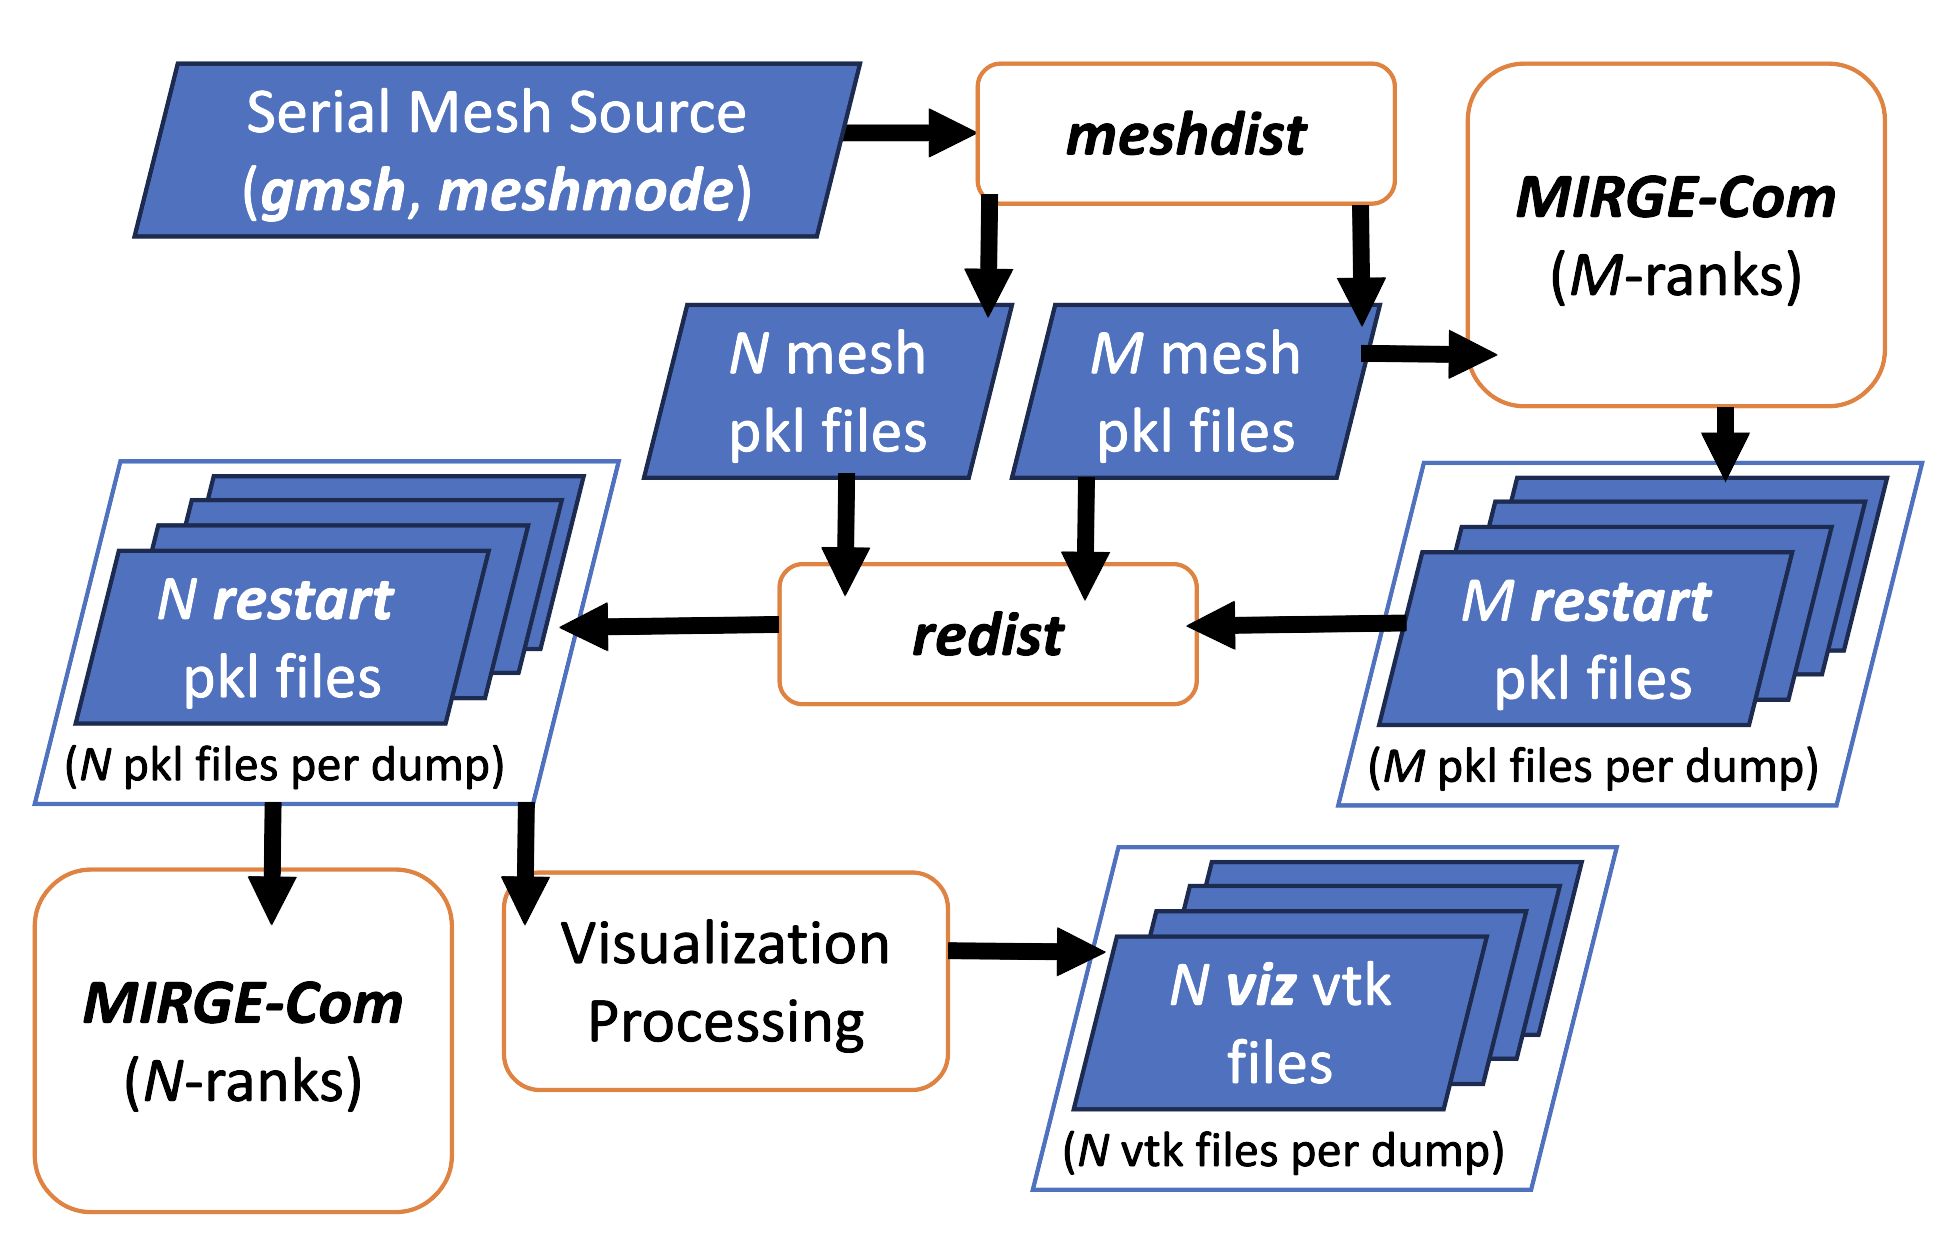
\includegraphics[width=\textwidth]{Figures/mtc/redist_data_flow_full.png}
\end{minipage}
\end{frame}

\begin{frame}\frametitle{M-to-N Transfer with \textit{redist}}
  \begin{minipage}[t][.4\textheight][t]{\textwidth}
    \begin{multicols}{2}
      \begin{itemize}
      \item Input: $M$-data (\mirgecom{} restart pkl files), $M$-decomp, $N$-decomp
      \item Unbonks the restart data with kludges:
        \begin{itemize}
        \item Detect DOFArrays in restart data: Must find an $M$-partition with \textit{all} volumes
        \item Compares DOFArray sizes to $M$-part volume sizes for volume-to-DOFArray correspondence
        \end{itemize}
      \item Creates DOFArray index mapping: $M$-decomp-local $\rightarrow$ $N$-decomp-local
      \item Reads and copies necessary $M$-data pkl files to cover $N$-part elements
      \item Writes $N$-data (new \mirgecom{} restart pkl files)
      \item Runs on arbitrary resource, dividing work like \textit{meshdist} 
      \end{itemize}
    \end{multicols}
  \end{minipage}
  \vfill
  \center{\texttt{redist.py -m 4 -n 3 -i rst\_4p -s mesh\_4p -t mesh\_3p -o rst\_3p}}
  \begin{minipage}[b][.4\textheight][t]{\textwidth}
    \begin{tikzpicture}[overlay, remember picture, scale=0.25]
      \node at (2cm, -14.5cm) (center) {};

      %\begin{scope}[shift={(center)}]  % yshift=-10cm]
      \begin{scope}[yshift=-12cm]
        % Partition (0,0)
        \draw[step=1, thin, black] (0,0) grid (4,10);
        \draw[thick] (0,0) rectangle (4,10);
        \node[font=\bfseries, blue] at (2,9) {(0,0)};
        
        % Partition (1,0)
        \begin{scope}[xshift=4.5cm]
          \draw[step=1, thin, black] (0,0) grid (4,10);
          \draw[thick] (0,0) rectangle (4,10);
          \node[font=\bfseries, blue] at (2,9) {(1,0)};
        \end{scope}

        % Partition (2,0)
        \begin{scope}[xshift=9cm]
          \foreach \i in {0,1,2,3} {
            \foreach \j in {3,4,...,9} {
              \draw (\i,\j) rectangle (\i+1,\j+1);
            }
          }
          \draw (0,0) rectangle (1,3);
          \draw (0,0) rectangle (1,1);
          \draw (0,1) rectangle (1,2);
          \draw (0,2) rectangle (1,3);
          \draw[thick] (0,0) -- (1,0) -- (1,3) -- (4,3) -- (4,10) -- (0,10) -- cycle;
          \node[font=\bfseries, blue] at (2,9) {(2,0)};
        \end{scope}

        % Partition (2,1) with blue subregion
        \begin{scope}[xshift=13.5cm, yshift=6cm]
          \draw[step=1, thin, black] (0,0) grid (2,4);
          \draw[thick] (0,0) rectangle (2,4);
          \foreach \j in {0,1,2,3} {
            \fill[blue] (0.5, \j+0.5) circle (4pt);
            \fill[blue] (1.5, \j+0.5) circle (4pt);
          }
          \node[font=\bfseries, blue] at (1,3) {(2,1)};
        \end{scope}

        % Partition (2,2) with red subregion
        \begin{scope}[xshift=13.5cm, yshift=2cm]
          \draw[step=1, thin, black] (0,0) grid (1,3);
          \draw[thick] (0,0) rectangle (1,3);
          \foreach \j in {0,1,2} {
            \fill[red] (0.5, \j+0.5) circle (4pt);
          }
          \node[font=\bfseries, blue] at (0.5,2) {(2,2)};
        \end{scope}

        % Partition (3,0)
        \begin{scope}[xshift=16cm, yshift=3.5cm]
          \draw[step=1, thin, black] (0,0) grid (4,7);
          \draw[thick] (0,0) rectangle (4,7);
          \node[font=\bfseries, blue] at (2,6) {(3,0)};
        \end{scope}
        
        % Partition (3,2) with red subregion
        \begin{scope}[xshift=16cm, yshift=-0.5cm]
          \draw[step=1, thin, black] (0,0) grid (4,3);
          \draw[thick] (0,0) rectangle (4,3);
          \foreach \j in {0,1,2} {
            \fill[red] (0.5, \j+0.5) circle (4pt);
            \fill[red] (1.5, \j+0.5) circle (4pt);
            \fill[red] (2.5, \j+0.5) circle (4pt);
            \fill[red] (3.5, \j+0.5) circle (4pt);
          }
          \node[font=\bfseries, blue] at (2,2) {(3,2)};
        \end{scope}
        \begin{scope}[xshift=40cm]
          % Partition (0,0)
          \draw[step=1, thin, black] (0,0) grid (5,10);
          \draw[thick] (0,0) rectangle (5,10);
          \node[font=\bfseries, orange] at (2.5,9) {(0,0)};

          % Partition (1,0) (panhandle grid)
          \begin{scope}[xshift=5.5cm]
            \foreach \i in {0,1,2,3,4} {
              \foreach \j in {3,4,...,9} {
                \draw (\i,\j) rectangle (\i+1,\j+1);
              }
            }
            \foreach \i in {0,1,2} {
              \foreach \j in {0,1,2} {
                \draw (\i,\j) rectangle (\i+1,\j+1);
              }
            }
            \draw[thick] (0,0) -- (3,0) -- (3,3) -- (5,3) -- (5,10) -- (0,10) -- cycle;
            \node[font=\bfseries, orange] at (2.5,9) {(1,0)};
          \end{scope}

          % Partition (1,1) with blue subregion
          \begin{scope}[xshift=9cm, yshift=-0.5cm]
            \draw[step=1, thin, black] (0,0) grid (2,3);
            \draw[thick] (0,0) rectangle (2,3);
            \foreach \j in {0,1,2} {
              \fill[blue] (0.5, \j+0.5) circle (4pt);
              \fill[blue] (1.5, \j+0.5) circle (4pt);
            }
            \node[font=\bfseries, orange] at (1,2) {(1,1)};
          \end{scope}

          % Partition (2,0)
          \begin{scope}[xshift=12cm, yshift=3cm]
            \draw[step=1, thin, black] (0,0) grid (6,7);
            \draw[thick] (0,0) rectangle (6,7);
            \node[font=\bfseries, orange] at (3,6) {(2,0)};
          \end{scope}

          % Partition (2,2) with red subregion
          \begin{scope}[xshift=12cm, yshift=-0.5cm]
            \draw[step=1, thin, black] (0,0) grid (6,3);
            \draw[thick] (0,0) rectangle (6,3);
            \foreach \j in {0,1,2} {
              \fill[red] (0.5, \j+0.5) circle (4pt);
              \fill[red] (1.5, \j+0.5) circle (4pt);
              \fill[red] (2.5, \j+0.5) circle (4pt);
              \fill[red] (3.5, \j+0.5) circle (4pt);
              \fill[red] (4.5, \j+0.5) circle (4pt);
              \fill[red] (5.5, \j+0.5) circle (4pt);
            }
            \node[font=\bfseries, orange] at (3,2) {(2,2)};
          \end{scope}
        \end{scope}
        \begin{scope}[xshift=8cm]
          % Coordinates for arrow
          \coordinate (leftGridCenter) at (8,5);
          \coordinate (rightGridCenter) at (38,5);
        
          % Arrow with text
          \draw[->, ultra thick] (leftGridCenter) -- node[midway, fill=white, text width=3cm, align=center] {\textit{redist}} (rightGridCenter);
        \end{scope}
      \end{scope}
    \end{tikzpicture}
  \end{minipage}
\end{frame}

\begin{frame}\frametitle{M-to-N Procedure Outline}
\begin{minipage}{0.49\textwidth}
\begin{itemize}
\item {\color{lightgray}{Generate the input mesh (\textit{gmsh} or built-in \textit{meshmode}})}
\item {\color{lightgray}{Create the target decompositions $M$,$N$}}
  \begin{itemize}
  \color{lightgray}
  \item Creates required mapping files
  \item Run \textit{meshdist} part to $M$, $N$ ranks
  \end{itemize}
\item {\color{lightgray}{Run \mirgecom{} on $M$ ranks}}
  \begin{itemize}
    \color{lightgray}
    %\item Example: Reading pre-generated mesh
  \item Generates $M$ restart files per dump
  \end{itemize}
\item {\color{lightgray}{Perform M-to-N transfer with \textit{redist}}}
\item Restart \mirgecom{} on $N$ ranks -or-
\item Post-processing/viz for $N$ ranks
\end{itemize}
\center{ ... Restart or post-process as usual.}
\end{minipage}
\hfill
\begin{minipage}{.49\textwidth}
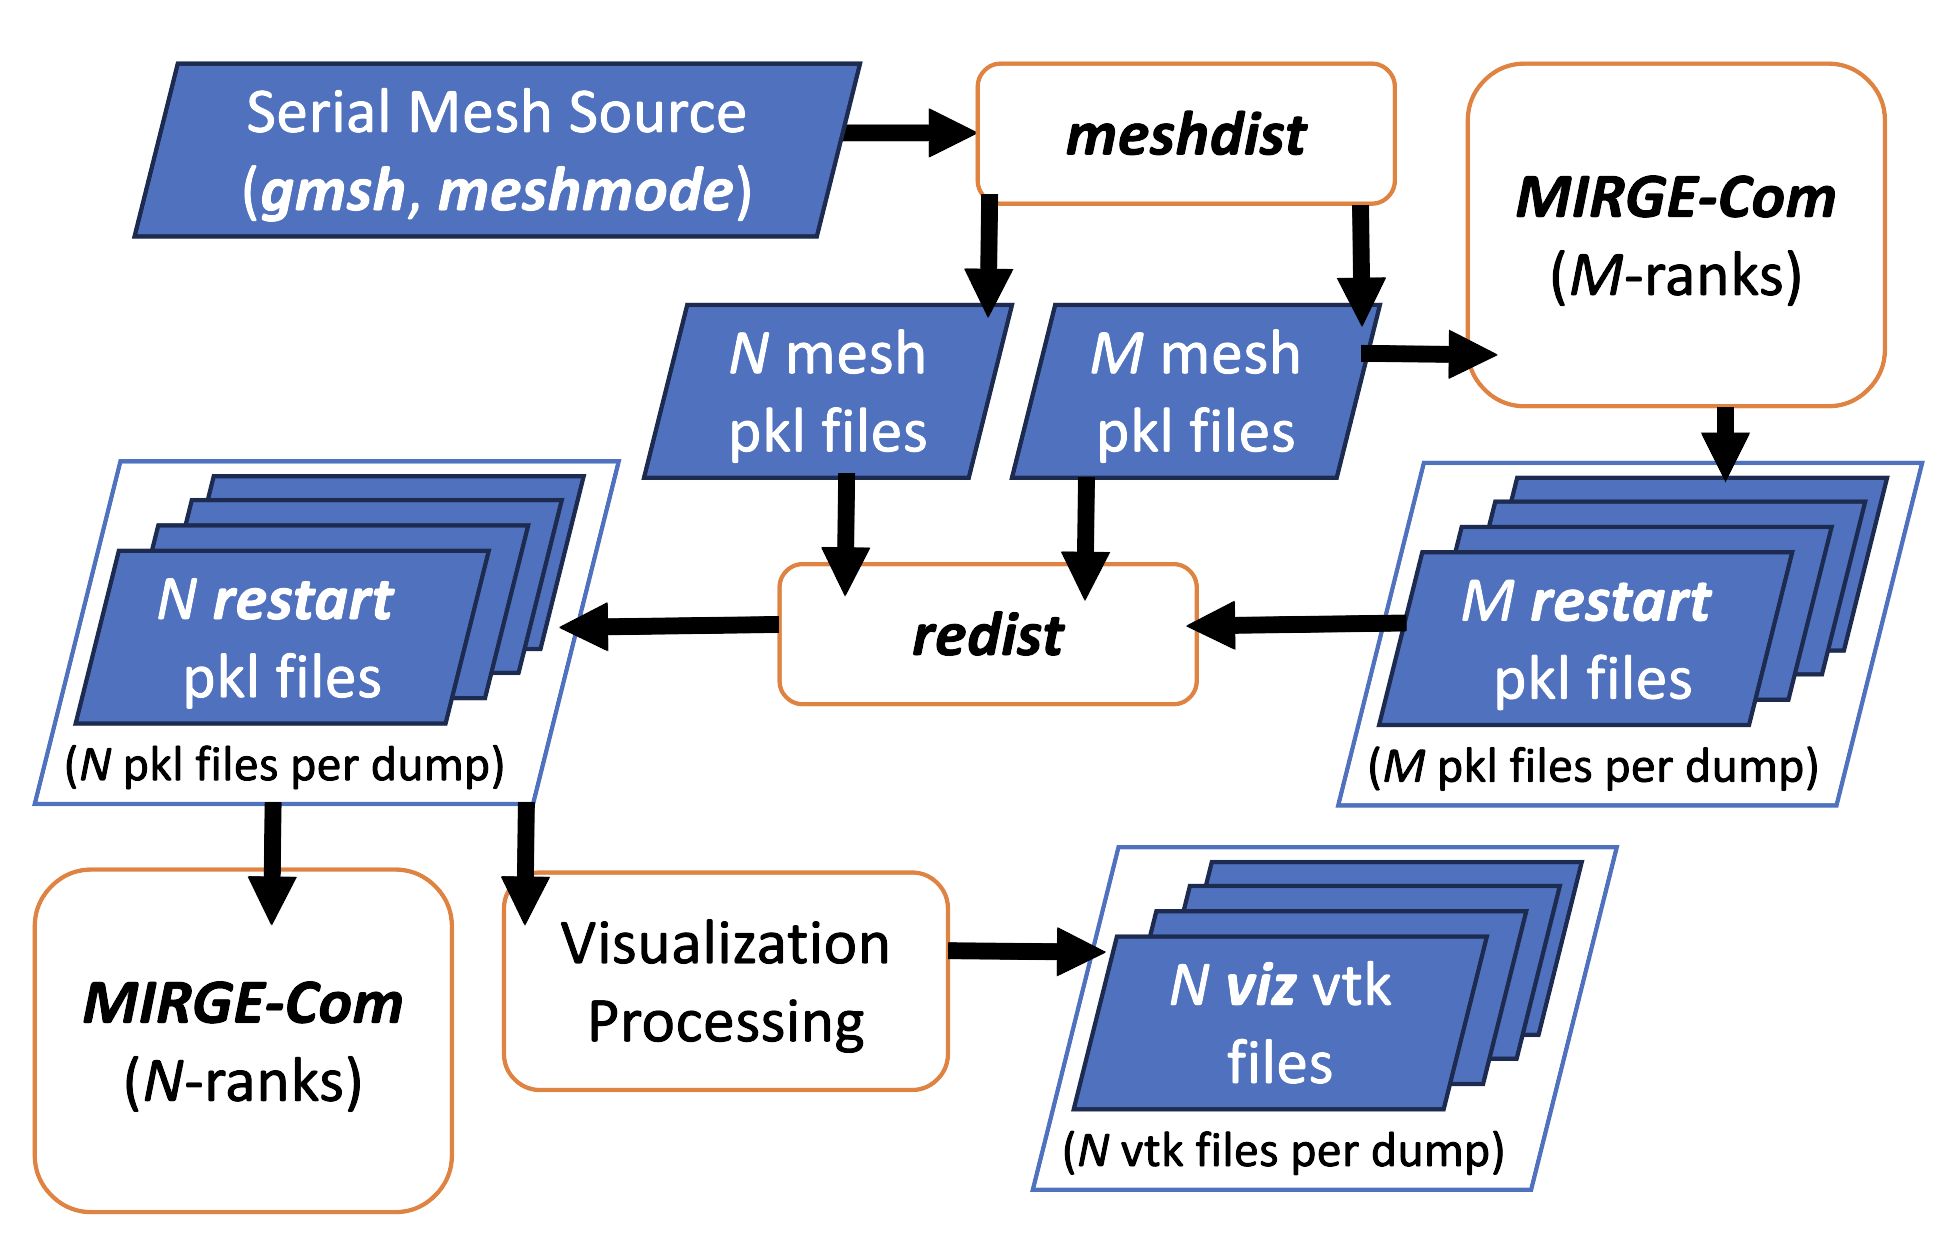
\includegraphics[width=\textwidth]{Figures/mtc/redist_data_flow_full.png}
\end{minipage}
\end{frame}

\begin{frame}\frametitle{TODOs For M-to-N}
  \begin{itemize}
  \item Everything is in \mirgecom{} PR 973 (WIP)
  \item Some things are prediction-specific (gmsh mesh source)
  \item Unkludge the restart debonk (some sort of standardization):
    \begin{itemize}
    \item Auto-detection of DOFArrays in restart data is OK - could be better
    \item Finding partition with all volumes, ugh
    \item Need some way to associate DOFArrays $\rightarrow$ Volume/dd
    \end{itemize}
  \item \textit{Meshmode} support for m-to-n mappings would be nice 
  \end{itemize}
\end{frame}


%======================================================================
\begin{frame}\frametitle{}

\vspace*{0.2in}

\begin{center}


\includegraphics[width=0.35\textwidth]{../ceesd-logo-2.pdf}

\vspace*{0.35in}
\cPI{\huge Questions?}

\vspace*{0.5in}
\begin{minipage}{0.6\textwidth}
This material is based in part upon work supported by the Department of Energy, National Nuclear Security Administration, under Award Number DE-NA0003963. 
\end{minipage}



\end{center}


\end{frame}
%======================================================================


\end{document}
